\newpage

\begin{figure}[h]
\centering
{\includegraphics[scale=.25]{0345.eps}}
\end{figure}

\begin{center}
{\large\bfseries{\sktf Ba;a:=+ti6a;a;ya;m,a A;Y3a;Da;Za;a;sa;na;m,a}}\\[10pt]
{\Large\bfseries{\sktf .sMa;s1k\ZH{-12}{\ZV{4}{x}}+:ta;a;ya;ea;gaH\ZS{4}}}%
\\[30pt]
{\Huge\bfseries{\sktf :pra:(\ZM{pFngFi}a;a;va;l\ZH{-8}{i9}+.a}}
\end{center}


\vskip 3cm

{\rm 
\begin{center}
{\large\bfseries{SANSKRIT COMMISSION}}\\[30pt]
{\large\bfseries{QUESTIONNAIRE}}
\end{center}
}

\vfill

\begin{center}
{\Large\bfseries{\sktf .sMa;s1k\ZH{-12}{\ZV{4}{x}}+:ta;a;ya;ea;ga \ZF{-}
.sa;Y4a;.ca;va;a;l+.yaH\ZS{4}}}\\
{\Large\bfseries{\sktf :pUa;na;a {\sktf 4}}}\\
{\large\bfseries{\sktf k+:a;Y5a:t1Ra;k \ZF{-} :pa;Ea;NRa;ma;a;si6a;a\ZF{,}
.sMa;va;t,a {\sktf 2013}\ZF{,} Za;k+:a;b.d;aH\ZS{4} {\sktf 1878}}}
\end{center}

\newpage

\begin{spacing}{1.15}
{{\sktf \ZS{12}@A\ZS{6}@A ?\ZS{12}@A\ZS{6}@A ;Y2a;va;Y2a;d;tMa Ka;l\ZH{-6}{u}
Ba;va;ta;Ma ya;t,a Ba;a:=+ta;ga;ta;s1ya .sMa;s1k\ZH{-12}{%
\ZV{4}{x}}+:ta;a;Dya;ya;na;s1ya .sa;a;m1\ZM{cLe}.pra;Y3a;ta;k\ZH{-12}{Y2}+:Ma
.sa;ma;va;s1Ta;Ma .sa;vRa;ta;ea;Y2a;d;ZMa :pa}{\sktf \ZS{0}:i8a:=+Zi6a;a;l+.Y4a;ya;tMua 1956 ;Y2a;k\ZM{l0R}+:s1ta;a;b.d;s1ya
A;k2+:ea;ba:=\ZF{-}ma;a;sea Ba;a:=+ti6a;a;yea;na A;Y3a;Da;Za;a;sa;nea;na}
`{\sktf .sMa;s1k\ZH{-12}{\ZV{4}{x}}+:ta;a;ya;ea;gaH\ZS{4}}'}

\vskip 0.1cm

{\sktf O;;SaH\ZS{4} A;a;ya;ea;gaH\ZS{4} .s1vi6a;a;ya;Y2a;va;Y2a;va;Da;k+:a;yeR%
a;Sua ;Y2a;va:(\ZM{dGu};a;Y2a;va;d\ZM{fByF0E};a;a;l+.ya;ga;tMa
ta;Y2a;d;ta:=+sMa;s1Ta;a;ga;tMa ..ca .sMa;s1k\ZH{-12}{%
\ZV{4}{x}}+:ta;Y5a;Za;[a;a;Y2a;va;Sa;ya;k\ZH{-12}{M} .sa;a}{\sktf mpra}{\sktf ;Y3a;ta;k+:m,a A;a;nua;k\ZH{-12}{U}+:l1yMa
;Y2a;va;l+.ea;k+:Y4a;ya;Sya;Y3a;ta\ZF{,} o+.pa;k+:l1pa;Y4a;ya;Sya;Y3a;ta ..ca
ta;Ma;s1ta;a;n,a o+.pa;a;ya;Y2a;va;Zea;Sa;a;n,a .sMa;s1k\ZH{-12}{%
\ZV{4}{x}}+:ta;a;Dya;ya;na;s1ya .sMa;s1k\ZH{-12}{\ZV{4}{x}}}{\sktf ta}{\sktf .sMa;Za;ea;Da;na;s1ya ..ca\break A;Y6a;Ba;v\ZV{4}{x}a:;d%
\ZM{t0Dj0b};yea \ZS{12}@A}

\vskip 0.1cm

{\sktf :pa:=+m1\ZM{cLe}.pa:=+a;ga;ta;Ma .sMa;s1k\ZH{-12}{%
\ZV{4}{x}}+:ta;Y5a;Za;[a;a;pra;Na;a;l\ZH{-8}{i9}+.Ma :pa:=\ZH{-6}{i7}+a;[ya
ta:t3a;tya;aH\ZS{4} :k\ZH{-12}{e} :k\ZH{-12}{e} ;Y2a;va;Zea;Sa;aH\ZS{4}
na;vi6a;a;na;Y5a;Za;[a;a;pra;Na;a;l1ya;a;m,a A{;nta}{Ba;Ra};v.ya;ma;a;na;aH\ZS{4} o+.pa;yua:j1yea:=+n,a\ZF{,} I+.tyea;ta;d;Y2a;pa
A;sa;Ea ;Y2a;va;.ca;a:=+Y4a;ya;Sya;Y3a;ta \ZS{12}@A}

{\sktf ta;m,a O;;nMa ;Y2a;va;Sa;ya;m,a A;Y3a;Da;k\ZH{-12}{\ZV{4}{x}}+:tya
ta;Y2a;d\ZM{oau};d;Ma ma;ta;m,a A;a;va;a;h;Y4a;ya;tua;m,a o+.pa;nya;s1ta;a
I+.yMa :pra;k\ZH{-12}{\ZV{4}{x}}+:tea;na A;a;ya;ea;gea;na
:pra:(\ZM{pFngFi}a;a;va;l\ZH{-8}{i9}+.a \ZS{12}@A I+.yMa ..ca :pra(\ZM{pFngFi}a;a;va;l\ZH{-8}{i9}+.a ;Y2a;va;pua;l+.Y2a;va;Sa;ya;a;va;ga;a;Y2a;h%
;ni6a;a \ZS{12}@A .tea;na ;Y2a;h\ZF{,} yea ma;h;a;Ba;a;ga;aH\ZS{4}
o+t1a:=+prea;Sa;Nea;na A;nua;Y6a:ja;G\ZV{4}{x}a;[ea;yuaH\ZS{4}\ZF{,} na
:tEaH\ZS{4} A;va;Zya{;mea;va} :pra;Y3a;ta;pr,aA:(\ZM{pFngFi}a;m,a o+t1a:=+m,a o+.d;a;h;a;yRa;m,a \ZS{12}@A ya:t3a
;Y2a;va;Sa;ya;Y2a;va;Zea;Sea yea;Sa;a;m,a A;Y6a;Ba;Y4a;na;vea;ZaH\ZS{4}
.sMa;ba;nDa;Y2a;va;Zea;SaH\ZS{4} va;a ;Y2a;va;Y5a;Za;S1\ZH{-6}{M} :]a;a;nMa
va;a .s1ya;a;t,a\ZF{,} ta:t3a .tea .s1va;ma;tMa ta;d\ZH{-10}{u};pa;ea;d\ZM{oaupabj0b};l+.k\ZH{-12}{M}
..ca yua;Y3a;k2+.ja;a;tMa .sa;ma;a;sea;na :pra;d;ZRa;yea;yuaH\ZS{4}\ZF{,}
I+.Y3a;ta .sa;veRa v.ya;va;h;ta;Ra:=\ZS{1}H\ZS{4} A;m1ya{;TyRa};ntea \ZS{12}@A
d\ZH{-6}{i6};a;ya;ma;a;nam,a o+t1a:=\ZH{-6}{M} :]a;a;pa;k\ZH{-12}{M} va;a yMa
:pra:(\ZM{pFngFi}a\ZH{-6}{M} .s1\ZM{cLe}.p\ZV{4}{x}a;Za;Y3a;ta\ZF{,} ta;s1ya
:pra:(\ZM{pFngFi}a;s1ya A;\ZM{0PqPOM0bvJbPJbEJdE}*:\ZS{2}H\ZS{4}
.s1\ZM{cLe}.pa;S1\ZH{-6}{M} ;Y4a;na;d\ZH{-6}{eR};ZyaH\ZS{4} \ZS{12}@A}

\vskip 0.1cm

{\sktf A;a:\ZM{FPqVOM00gFEILdlXDI}*+:+.Ba;a;Sa;ya;a
.sMa;s1k\ZH{-12}{\ZV{4}{x}}+:ta;Ba;a;Sa;ya;a va;a o+t1a:=+a;Y5a;Na
d;a;ta;v.ya;a;Y4a;na \ZS{12}@A o+t1a:=+a;Y5a;Na ..ca} `{\sktf
.sa;d;s1ya\ZF{-}.sa;Y4a;.ca;vaH\ZS{4}\ZF{,} .sMa;s1k\ZH{-12}{%
\ZV{4}{x}}+:ta;a;ya;ea}{\sktf ga.h}, {\sktf :pUa;na;a 4}' {\sktf O;;ta;m,a o+.Y1a;d1+Zya ta;Ta;a
:prea;Sa;Ni6a;a;ya;a;Y4a;na\ZF{,} ya;Ta;a 12 ;Y2a;q+.sa;m1ba:=\ZF{,} 1956
O;;ta;t,a ;Y2a;d;nMa ya;a;va;t,a :pra;a;pyea:=+n,a \ZS{12}@A}

\vskip 0.1cm

{\sktf I+.d\ZH{-6}{M} ..ca A;pa:=\ZH{-6}{M} v.ya;va;h;ta;Ra:=\ZS{1}H\ZS{4}
:pra;a;TyRa;ntea\ZF{,} ya;t,a .tea .s1vea;Sa;a;m,a o+t1a:=+a;Na;a;m,a
A;va;sa;a;nea ;Y4a;na:jMa .sa;ma;gr4Ma na;a;ma\ZF{,} A;Y3a;Da;k+:a:=+m,a\ZF{,}
A;a;vaA;sa;s1Ta;a;nMa ..ca ;Y4a;l+.Kea;yuaH\ZS{4} \ZS{12}@A\ZS{6}@A}
\end{spacing}
\medskip

{\rm 
You are aware that the Government of India have appointed (in October 1956) a Sanskrit Commission to consider the question of the present state of Sanskrit Education in India.

\vskip .1cm

The commission will, among other things survey the existing facilities for Sanskrit Education in Universities and non-University institutions and make proposals for promoting the study of Sanskrit, including research, It will also examine the traditional system of Sanskrit Education in order to find out what features from it an be usefully incorporated into the modern system.


With a view to eliciting informed public opinion on the subject, the Commission has issued the present Questionnaire. The Questionnaire convers a wide field of inquiry, and it is not intended that all those who are pleased to send replies should necessarily answer every question. Correspondoents are requested to favour the Commission with their views and suggestions on matters in which they are particulary interested or concerrxed, or of, which they have special knowledge. Reasons, in brief, may please be given in support of the views expressed. The number of the question to which the answer or memorandum relates should be clearly indicated.

Replies, in English or Sanskrit, may be kindly sent to `The Member Secretary, Sanskrit Commission, Poona 4', so as to reach him not later than the 12th of December, 1956. 

Correspindents are requested to give their full names, designations, and addresses at the end of their replies.
}

\newpage

\begin{spacing}{1.15}
{\sktf \ZS{12}@A\ZS{6}@A A \ZS{12}@A\ZS{6}@A .sa;a;ma;a;nya;pra;k+.=+Na;m,a
\ZF{-} mUa;l+.BUa;ta;aH\ZS{4} :k\ZH{-12}{e}+:.ca;na
:pra:(\ZM{pFngFi}a;aH\ZS{4} \ZS{12}@A\ZS{6}@A}

\begin{itemize}
  \item[{\sktf 1}.] {\sktf k+:a BUa;Y6a;ma;k+:a k+:a;yRa;Y2a;va;Zea;SaH\ZS{4}
va;a .sMa;s1k\ZH{-12}{\ZV{4}{x}}+:ta;Y2a;va;d;a A;d\ZM{fByF0E};a;ta;nea
Ba;a:=+ta;s1ya .=+a;Y2a;S1\ZH{-10}{r1};ya:ji6a;a;va;nea
;Y4a;na;vRa;tRa;Y4a;ya;ta;v.y,aAH\ZS{4} \ZF{?}}  
  
  \item[{\sktf 2}.] \begin{itemize} 
    \item[({\sktf k})] {\sktf .sMa;s1k\ZH{-12}{\ZV{4}{x}}+:ta;a;Dya;ya;nMa
:pra;Y3a;ta Ba;va;d\ZH{-6}{i6};a;yea k\ZH{-12}{Y2}+:a;d\ZH{-4}{%
\ZV{2}{x}};Zi6a;a .ja;na;a;na;Ma .sa;a;Da;a:=+Ni6a;a
ma;na;ea;v\ZV{4}{x}a;Y5a:t1aH\ZS{4} \ZF{?}}
                        
    \item[({\sktf Ka})] {\sktf :pa;a;F+.Za;a;l+.a;sua\ZF{,}
ma;h;a;Y2a;va;d\ZM{fByF0E};a;a;l+.yea;Sua\ZF{,} ;Y2a;va:(\ZM{dGu};a;Y2a;va;d%
\ZM{fByF0E};a;a;l+.yea;Sua ..ca :pra;va;tRa;ma;a;na;a;t,a
.sMa;s1k\ZH{-12}{\ZV{4}{x}}+:ta;a;Dya;ya;na;a;t,a {v.ya};Y3a;ta;=\ZH{-6}{e}+k\ZH{-12}{e}+:Na\ZF{,} ;k\ZH{-12}{E}\ZS{3}H\ZS{4}
;k\ZH{-12}{E}\ZS{3}H\ZS{4} o+.pa;a;ya;a;nta;=\ZH{-6}{E}\ZS{1}H\ZS{4}
Ba;va;d\ZH{-6}{i6};a;yea :pra;d\ZH{-6}{e};Zea .sMa;s1k\ZH{-12}{%
\ZV{4}{x}}+:ta;Y2a;va;d\ZM{fByF0E};a;a;ya;aH\ZS{4}
A;Y6a;Ba;v\ZV{4}{x}a;Y4a:;d\ZM{t0Dj0b}H\ZS{4} ;Y2a;k\ZM{l0R}+:ya;tea\ZF{,}
.sMa;s1k\ZH{-12}{\ZV{4}{x}}+:ta;sa;a;Y2a;h;tyea ta;d;n,ao+.pra;a;Y5a;Na;ta;a;ya;Ma .sMa;s1k\ZH{-12}{\ZV{4}{x}}+:ta;Ea ..ca
A;a;d:=\ZS{1}H\ZS{4} :pa;i8a:=+pa;a;l1ya;tea \ZF{?,}
I\ZH{-6}{R}+.d\ZH{-4}{\ZV{2}{x}};Za;s1ya A;a;d:=+s1ya
A;Y6a;Ba;v\ZV{4}{x}a:;d\ZM{t0Dj0b}\ZH{-6}{e};(\ZM{rac0FI}a A;TeRa
:k\ZH{-12}{e} o+.pa;a;ya;aH\ZS{4} Ba;va;Y5a;;d2\ZM{x0Bi0ed0E}\ZS{1}H\ZS{4}
.sUa;.cyantea \ZF{?}}
     \end{itemize}
                       
 \item[{\sktf 3}.] \begin{itemize}
      \item[({\sktf k})] {\sktf ma;a;na;Y2a;va;k\ZH{-12}{Y2}+:a
.sa;Ma;s1k\ZH{-12}{\ZV{4}{x}}+:Y3a;ta;k\ZH{-12}{Y2}+:a ..ca
.sMa;s1k\ZH{-12}{\ZV{4}{x}}+:ta;s1ya A;na;GRa;ta;a;m,a A;a;l+.ea;.cya\ZF{,}
.sMa;s1k\ZH{-12}{\ZV{4}{x}}+:ta;a;Dya;ya;na ;Y2a;va;Sa;yea ma{;h\ZH{-6}{i6};a}}{\sktf yaH\ZS{4}} {\sktf o+;d\ZM{t0Dj0b};ea;Da;na;m,a A;a;d:=\ZH{-6}{M} ..ca
Ba;a:=+ti6a;a;ya ga;Na;ta:n:t4a;a;nua;pa;a;Y4a;l+.tea;Sua
na;a;ga;i8a:=+k\ZH{-12}{e}+:Sua .sa;mua;tpa;a;d;Y4a;ya;tMua k+:a;n,a
o+.pa;a;ya;a;n,a o+.pa;a;d\ZH{-6}{e}ya;tvea;na Ba;va;ntaH\ZS{4} .sUa;.ca;yea;yuaH\ZS{4}\ZF{?}}
                      
 \item[({\sktf Ka})] {\sktf k\ZH{-12}{Y2}+:a;d\ZH{-4}{\ZV{2}{x}};%
\ZH{0}{i0//////Y7}a;gBaH\ZS{4} ;Y2a;va;Da;a;Y6a;BaH\ZS{4}} `{\sktf
.sa;a;Y2a;h;tya \ZF{-} A;k+:a;d\ZH{-6}{e};mi6a;a}' {\sktf
\ZF{(}A;\ZH{0}{i0Y7}a;Ka;l\ZF{-}Ba;a:=+ti6a;a;ya\ZF{-}.sa;a;Y2a;h;tya%
\ZF{-}:pa;i8a:=+Sa;t,a\ZF{)} .ja;na;a;na;Ma} {\sktf .sMa;s1k\ZH{-12}{\ZV{4}{x}}+:ta;va;a:%
\ZM{0PqPOMDbmQbiX0AXhA}*+;;ya;a;Dya;ya;na;s1ya} {\sktf
:pra:=+ea;.ca;na;a;ya\ZF{,} ta;Y2a;d\ZM{oau};Sa;yea ..ca
A;a;d:=+sMa;va;DRa;na;a;ya\ZF{,} .sa;a;h;a;yyMa} {\sktf ktR2ua Za;\ZM{0NkLNPLPE0DnLDE}*:\ZH{-8}{\ZV{-2}{u}}+:ya;a;t,a \ZF{?} .tea;Sua
.tea;Sua ;Y2a;va;d\ZM{fByF0E};a;a;s1Ta;a;nea;Sua :pra;Y3a;ta;Y4a;na;Y3a;Da;BUa%
;ta;a;na;Ma .sMa;s1k\ZH{-12}{\ZV{4}{x}}+:ta;gr4a;nTa;a;na;a;m,a \ZF{(}1\ZF{)}
A;a:\ZM{FPqVOM00gFEILdlXDI}*+:+.Ba;a;Sa;a;ya;Ma \ZF{(}2\ZF{)}
:pra;a{;d\ZH{-6}{e}};Y5a;Za;k+:Ba;a}{\sktf :Sa;a;sua} {\sktf ..ca A;nua;va;a}{\sktf
;d\ZH{-6}{E}H\ZS{4}} {\sktf .sa;h;k\ZH{-12}{\ZV{4}{x}}+:ta;a;Y4a;na
.s1va;l1pa;mUa;l1ya;a;Y4a;na .sMa;s1k+.=+Na;a;Y4a;na
:k\ZH{-12}{e}+:nd\ZP{-8}{-4}{@R}+a;Y3a;Da;Za;a;sa;na;s1ya} {\sktf .=+a:j1ya;a;Y3a;Da}{\sktf Za;a;sa;na;a;na;Ma} {\sktf ..ca
d\ZM{oau};a:=\ZH{-6}{e}+Na}  `{\sktf .sa;a;Y2a;h;tya\ZF{-}A;k+:a;d%
\ZH{-6}{e};mi6a;a}' {\sktf .s1va;yMa :pra;k+:a;Za;yea;t,a A;nyEaH\ZS{4} va;a :pra;k+:a;Zya;ma;a;na;a;Y4a;na :pua:=+s1k\ZH{-12}{u}+:ya;Ra;t,a\ZF{,}
I+.tyea;ta;Y2a;d\ZM{oau};Sa;yea Ba;va;ta;Ma ;Y2a;k\ZH{-12}{M} ma;ta;m,a\ZF{?}}
[{\sktf ya;va;na\ZF{-}.=+ea;ma;k\ZF{-}Ba;a;Sa;ya;eaH\ZS{4}
;Y4a;l+.\ZH{0}{i0Y7}a;Ka;ta;a;na;Ma gr4a;nTa;a;na;a;m,a {A;a:\ZM{FPqVOM00gFEILdlXDI}*+:}+.Ba;a;Sa;a;nua;va;a;d\ZF{-}.sa;h;k\ZH{-12}{%
\ZV{4}{x}}+:ta\ZF{-}.sMa;s1k+.=+Na;a;na;Ma :pra;Na;ya;nea\ZF{,}} `{\sktf
l+.ea.O;;ba\ZF{-}{\break}\ZM{0NkLNPLPELFI00l}*:+:a;Y6a;sa;k+:l%
\ZF{-}l+.a;ya;b.ra:=\ZH{-6}{i7}+a}' {\sktf .sMa{;s1Ta}ya;a ya;a .sa:=+a;Ni6a;aH\ZS{4} A;nua;\ZH{0}{i0Y7}a;s1\ZM{aLeDDr}:a;ya;tea%
\ZF{,} .sa;a A:t3a o+.d;a;h;a;ya;Ra \ZS{12}@A}\,]
                      
\item[({\sktf ga})] {\sktf ;Y2a;d\ZM{oau};ti6a;a;ya;s1ya;Ma
:pa;a:\ZM{BNz0dcRfA}*.a;va;Y2a;SRa;ky2+.a;Ma ya;ea:ja;na;a;ya;Ma
.sMa;s1k\ZH{-12}{\ZV{4}{x}}+:ta;Y5a;Za;[a;a;ya;aH\ZS{4}
A;Y6a;Ba;va;DRa;na;a;ya :k\ZH{-12}{e} o+.pa;a;ya;aH\ZS{4} Ba{va};nm1\ZM{cLe}.a;tea A;va;l+.m1ba;ni6a;a;ya;aH\ZS{4} \ZS{12}@A}
 \end{itemize} 
\end{itemize}
\end{spacing}

{\rm 
\section*{{\rm\bfseries A. General-Some Basic Questions}}

\noindent
\begin{itemize}
  
  \item[1.] What special role has Sanskrit to play in the national life of India to-day?
  
  \item[2.] \begin{itemize}
            \item[(a)] How would you characterize the general sentiment in your part of the conuntry towards the study of Sankrit?  
              
              \item[(b)] Apart from its study in P$\bar{a}$tha$\acute{s}\bar{a}$l$\bar{a}$s, Colleges and Universities, in what other ways are the cultivation of Sanskrit and interest in its literature and culture maintained in your part of the country? What steps would you suggest to promote such interest and cultivation?
             \end{itemize}
  \item[3.]\begin{itemize}
           \item[(a)] In view of the humanistic and cultural value of Sanskrit what steps would you sugeest for engendering among the citizens of the Republic of India a greater awareness for and interest in the study of Sanskrit?
           
           \item[(b)] In what ways can the {\textit {Sahitya Akademi}} help to popularize and promote interest in the study of Sanskrit literature? Should the {\textit {Sahitya Akademi}} in your opinion, undertake and encourage the publication by the Center as well as the States, in cheap editions, of representative Sanskrit texts in the different branches of learning, with accompanying translations in (i) English and (ii) the regional languages (in a style like that of the {\textit {Loeb Classical Library}} of Greek and Latin texts in English, for example)?
           
           \item[(c)] What provisions, in your opinion, need be made in the Second Five Year Plan for the promotion of Sanskrit Education?
           \end{itemize}
\end{itemize}           
}
\begin{spacing}{1.15}
\begin{itemize}
\item[{\sktf 4}.] \begin{itemize}
  \item[({\sktf k})] {\sktf A;pyea;ta;t,a Ba;va;ta;a;m,a A;Y6a;Ba;ma;tMa
ya;t,a k+:sma;a;Y5a;c1a;d;Y2a;pa Ba;a:=+ti6a;a;ya;a;t,a
;Y5a;Za;[a;a;pi6a;a;F+.a;t,a .sa;ma;a;va;tRa;ma;a;nea;na yua{;va}.ja;nea;na .sMa;s1k\ZH{-12}{\ZV{4}{x}}+:ta;sMa;s1k\ZH{-12}{\ZV{4}{x}}+:teaH%
\ZS{4} bi6a;a:ja;BUa;tEaH\ZS{4} A;\ZM{0PqPOM0bgNaENdE}*:\ZH{-8}{E}\ZS{2}H%
\ZS{4} A;va;Zya;m,a A;a:t1a :pa;i8a:=+.ca;yea;na Ba;Y2a;va;ta;v.ya;m,a
I+.Y3a;ta\ZF{?}}
                
   \item[({\sktf Ka})] {\sktf :k\ZH{-12}{e} :k\ZH{-12}{e} o+.pa;a;ya;aH\ZS{4}
Ba;va;tMa .sMa;ma;ta;aH\ZS{4} .yEaH\ZS{4} A;a;d\ZH{-4}{\ZV{2}{x}};tEaH\ZS{4}
;Y2a;va;d\ZH{-6}{e};Za;ga;a;Y6a;ma;naH\ZS{4} ba;h;vaH\ZS{4} C+.a:t3a;aH\ZS{4}
A;Y3a;Da;k+:a;i8a:=:NaH\ZS{4}\ZF{,} Ba;a:=+ta:=+a;Y2a;S1\ZH{-10}{r1};ya;k+:a;ya;Ra;l+.yea;Sua
;Y4a;na;yua;k2+:aH\ZS{4}\break k+:mRa;.ca;a;i8a:=+Na;(\ZM{rac0FI}a\ZF{,}
nyUa;na;a;Y3a;Da;k+:ya;a ma;a:t3a;ya;a O;;ta;s1ya;aH\ZS{4}
.sMa;s1k\ZH{-12}{\ZV{4}{x}}+:teaH\ZS{4} ya;Ta;aTRa;tvea;na :pa;i8a:=+.ca;a;ya;k+:aH\ZS{4} Ba;vea;yuaH\ZS{4}\ZF{?}}
                
 \item[({\sktf ga})] {\sktf A;pyea;ta;t,a Ba;va;ta;Ma ma;ta;m,a\ZF{,} ya;t,a
;Y2a;va;d\ZH{-6}{e};Za;s1Tea;Sua Ba;a:=+ti6a;a;ya\ZF{-}.=+a:ja;d%
\ZH{-10}{U};ta;a;va;a;sea;Sua .sMa;s1k\ZH{-12}{\ZV{4}{x}}+:ta
;Y2a;va;d\ZH{-10}{u};Sa;Ma ;Y4a;na;yua;k\ZH{-12}{,};Y3a;taH\ZS{4} ;Y2a;k\ZM{l0R}+:ya;tea ..cea;t,a\ZF{,}
.=+a:ja;d\ZH{-10}{U};ta;a;va;a;sa;ga;ta;a;Y4a;na .sa;Ma;s1k\ZH{-12}{%
\ZV{4}{x}}+:Y3a;ta;k+:a;Y4a;na A;Dya;va;Y6a;sa;ta;a;Y4a;na .sa;Ea;k+:yRa;m,a
A;a;pa;ts1ya;ntea I+.Y3a;ta\ZF{?}}
\end{itemize} 
           
 \item[{\sktf 5}.]  {\sktf ;Y4a;na;\ZH{0}{i0Y7}a;Ka;l+.Ba;a:=+ti6a;a;yea;Sua
:k\ZH{-12}{e}+:Sua;Y4a;.ca;t,a A;a;Y3a;Da;k+:a;i8a:=+k\ZH{-12}{e}+:Sua
v.ya;va;h;a:=\ZH{-6}{e}+Sua\ZF{-}.sa;a;Da;a:=+Na;Y2a;va;Sa;ya;a;n,a
A;Y3a;Da;k\ZH{-12}{u}+:va;Ra;NaH\ZS{4} A;a{;nta}.=;=+a:j1yi6a;a;yaH\ZS{4} l\ZH{-8}{e}+.Ka;v.ya;va;h;a:=\ZS{1}H\ZS{4}\ZF{,}
A;Ea;tsa;Y2a;va;k+:aH\ZS{4} ..ca :pra;sa;\ZM{0PqPOM0bgNaENdE}*:+.aH\ZS{4}
;Y2a;va:(\ZM{dGu};a;Y2a;va;d\ZM{fByF0E};a;a;l+.ya\ZF{-}.=+:%
\ZM{rMolHneHegMi}a;a;ta;k+:a;nua;Za;a;sa;na;m,a\ZF{,} Za;pa;Ta;pa;a;F+.na;m,a
Ba;a:=+ti6a;a;ya}-{\sktf ga;Na;ta:n:t4a;s1ya k\ZH{-12}{\ZV{4}{x}}+:tea
;vEa;d\ZH{-6}{e};Y5a;Za;k+:Za;a;sa;na;a;Y4a;na o+.Y1a;d1+Zya
.sMa;d\ZH{-6}{e};ZaH\ZS{4}\ZF{,} I+.tyea;va;ma;a;Y2a;d;Sua\ZF{-}}{\sktf
.sMa;s1k\ZH{-12}{\ZV{4}{x}}+:ta;s1ya o+.pa;ya;ea;gaH\ZS{4}
Ba;va;Y5a;;d2\ZM{x0Bi0ed0E}\ZS{1}H\ZS{4} .sMa;Ba;a;v.ya;tea ;Y2a;k+:m,a\ZF{?}}
 
 \item[{\sktf 6}.]  `{\sktf ;Da;mRa;Y5a;Za;[a;a;m,a}' {\sktf
A;Y3a;Da;k\ZH{-12}{\ZV{4}{x}}+:tya} `{\sktf ;Y2a;va:(\ZM{dGu};a;Y2a;va;d%
\ZM{fByF0E};a;a;l+.ya\ZF{-};Y5a;Za;[a;a;ya;ea;gea;Na}' {\sktf
;Y2a;va;Y2a;h;ta\ZF{-}:pUa{;va;Ra}{:Na;Ma}} {\sktf ZMa;sa;na;a;na;Ma ;Y4a;na;va;Ra;h\ZH{-6}{e}\ZF{,}} {\sktf
.sMa;s1k\ZH{-12}{\ZV{4}{x}}+:ta;a;Dya;ya;nMa :k\ZH{-12}{e}+:na ma;a;geRa;Na
o+.pa;ya;ea;Y3a;ga;ta;a;m,a A;va;a;p\ZM{lBn0BE}a\ZH{-6}{\ZV{-4}{u}};ya;a;t,a%
\ZF{?}} [{\sktf A;\ZH{0}{i0/////////Y7}a;sma;n,a ;Y2a;va;Sa{yea} d\ZP{-8}{-4}{@R}+S1;v.ya;m,a}{\rm ---} `{\sktf
;Y2a;va:(\ZM{dGu};a;Y2a;va;d\ZM{fByF0E};a;a;l+.ya\ZF{-};Y5a;Za;[a;a;ya;ea;ga;s%
1ya :pra;vea;d;na;m,a},' {\sktf :pra;Ta;maH\ZS{4} Ba;a;gaH\ZS{4} 1949\ZF{,}
:p\ZV{4}{x}a;S2+m,a 303 \ZS{12}@A}\,]   
 
 \item[{\sktf 7}.] \begin{itemize}
  \item[({\sktf k})]  {\sktf A;\ZH{0}{i0Y7}a;Ka;l\ZH{-8}{e} Ba;a:=+tea
.sMa;s1k\ZH{-12}{\ZV{4}{x}}+:ta;ea;c1a;a:=+Na;s1ya O;;k+.r9+.pa;ta;Ma
v.ya;va;s1Ta;a;pa;Y4a;ya;tMua .tea;Sua .tea;Sua :pra;d\ZH{-6}{e};Zea;Sua Ba{;va}nm1\ZM{cLe}.a;tea :k\ZH{-12}{e} :k\ZH{-12}{e} o+.pa;a;ya;aH\ZS{4}
A;va;l+.m1ba;ni6a;a;ya;aH\ZS{4}\ZF{?}} 
            
  \item[({\sktf Ka})] {\sktf .sMa;s1k\ZH{-12}{\ZV{4}{x}}+:ta;s1ya
mua;d\ZP{-8}{-4}{@R}+Nea l\ZH{-8}{e}+.Ka;nea ..ca .sa;vRa:t3a
O;;k+:s1ya;aH\ZS{4} O;;va ;Y4a;l+.peaH\ZS{4} .s1vi6a;a;k+.=+NMa
\ZF{(}ya;Ta;a\ZF{,} :d\ZH{-6}{e};va;na;a;ga;ya;RaH\ZS{4}\ZF{)} \ZF{(}1\ZF{)} A;\ZH{0}{i0Y7}a;Ka;l\ZF{-}Ba;a:=+ti6a;a;ya%
\ZF{-}v.ya;va;h1+.Y3a;ta;Sua\ZF{,} \ZF{(}2\ZF{)} ta:t1a;ts1Ta;a;ni6a;a;ya%
\ZF{-};Y4a;l+.pya;nta:=+a;Y5a;Na :pra;yua:\ZM{BNz0djR0ARdA}*+;a;nea;Sua
.=+a:j1ya;a;nta:=\ZH{-6}{e}+Sua ..ca ya;Ta;a;k{+:Ta};ma{;Y2a;pa}} {\sktf .sMa;s1k\ZH{-12}{\ZV{4}{x}}}{\sktf {ta;a};Dya;ya;na;sa;mua;n1a;teaH%
\ZS{4}} {\sktf .sa;a;Da;k\ZH{-12}{M} Ba;Y2a;va;Sya;Y3a;ta ;Y2a;k+:m,a\ZF{?}
ta;a;s1ta;aH\ZS{4} :pra;a;d\ZH{-6}{e};Y5a;Za;ky2+.aH\ZS{4} ;Y4a;l+.pyaH\ZS{4}
\ZF{(}va;\ZM{0PqPOM0bgNaENdE}*:\ZH{-8}{i9}+.a{;ya;a}\ZF{,} A;a;nDri6a;a;ya;a\ZF{,} k+:Na;Ra;f\ZH{-8}{i7};a;ya;a\ZF{,}
I+.tyea;va;ma;a;d\ZM{fByF0E};a;aH\ZS{4}\ZF{)} ta;tpra;ya;ea;Y3a;ga;Ni6a;a;na;M%
a :pra;a;d\ZH{-6}{e};Y5a;Za;k+:Ba;a;Sa;a;Na;Ma .sMa;s1k\ZH{-12}{%
\ZV{4}{x}}+:ta;Ba;a;Sa;ya;a .sMa;ba;nDMa {d\ZP{-8}{-4}{@R}}Q{+Y4a;ya};tua;m,a\ZF{,} ta;TEa;va ta;tpra;ya;ea;Y3a;ga;NaH\ZS{4} .ja;na;a;n,a
.sMa;s1k\ZH{-12}{\ZV{4}{x}}+:tea;na :pa;i8a:=+Y4a;.ca;ta;ta:=+a;n,a
;Y2a;va;Da;a;tua;m,a\ZF{,} ;Y2a;k+:ya;nm1\ZM{cLe}.a;a:t3a;m,a
o+.pa;k+:a;i8a:=+NyaH\ZS{4} Ba;va;\ZH{0}{i0////Y7}a;nta I+.Y3a;ta Ba{;va}ntaH\ZS{4} ma;nya;ntea\ZF{?}}
	
 \end{itemize}
\end{itemize}
\end{spacing}

{\rm 
\begin{itemize}
\item[4.] \begin{itemize}
             \item[(a)] Do you think that a young person who has passed out of an Indain Educational Institution should necessarily possess some grounding in the elements of Sanskrit culture? 
             
             \item[(b)] What steps need to be taken to enable the numerous Indian Students, Officials, and Employes of Indian establishments going to foregin countries to become, in some measure, true interpreters of this culture?
             
             \item[(c)] Do you think that the employement of Sanskrit scholars in Indian Embassies abroad will facilitate the cultural activities of those Embassies?
             \end{itemize}
             
\item[5.] What are the possibilities of the use of Sanskrit for the purpose of certain official matters of an all-India character, e.g. interstate communication on general topics, state and ceremonial occasions, University convocations, administration of oaths, and addressing foreign states on behalf of the Republic of India ?  
  
  \item[6.] In what can the study of Sanskrit be made serviceable in the implementations of the recommendations made by the University Education Commission regarding `Religious Education' (vide {\textit {Report of the University Education Commission}}, Vol.I, 1949, p.303)? 
  
  \item[7.] \begin{itemize}
            \item[(a)] What stepts would you suggest for securing uniformity of pronunciation in Sanskrit on an all-India basis for the various parts of the country?
            \item[(b)] Will the universal adoption of a single script (e.g. the Devanagari) in printing as well as writing Sanskrit in any way help promotion of Sanskrit studies (i) in all India contexts, and (ii) in the various States using local scripts? How far do you think are the various regional scripts (like Bengali, Telugu, Kannada. etc.) helpful in strengthening the close relation between Sanskrit and the regional languages using those scripts and in bringing  Sanskrit nearer to peoples using them?
            \end{itemize}
\end{itemize}
}

\begin{spacing}{1.15}
\begin{itemize} 
\item[] \begin{itemize}
          \item[({\sktf ga})] {\sktf A;pyea;ta;t,a Ba;va;ta;Ma ma;ta;m,a\ZF{,}
ya;t,a .sa:=+l\ZH{-8}{i9}+.a;k\ZH{-12}{\ZV{4}{x}}+:ta;s1ya mUa;l+.BUa;ta;s1ya
va;a .sMa;s1k\ZH{-12}{\ZV{4}{x}}+:ta;s1ya ;Y2a;va;k+:a;sa;nMa .sMama;TTeRa I+.Y3a;ta \ZF{?} ya;Y2a;d O;;va;m,a\ZF{,} k+:aH\ZS{4} Ba;va;ta;Ma
;Y2a;d;Sa;yea .sUa;.ca;na;aH\ZS{4} \ZF{?}}
          \end{itemize}                                         
          
\item[{\sktf 8}.]  \begin{itemize}
   \item[({\sktf k})] {\sktf ;Y5a;Za;[a;a;ya;aH\ZS{4}
l+.ea;k+:sea;va;a;ya;a;(\ZM{rac0FI}a [ea:t3ea\ZF{,}
:pra;d;ea;Y5a;Za;k+:Ba;a;Sa;a;ya;aH\ZS{4} o+.pa;ya;ea;gaH\ZS{4}
.sMa;pra;Y3a;ta .sa;Y4a;na;bRa;nDa;m,a o{+.pa}{:pa;a}{d\ZM{fByF0E};a};ma;a;naH\ZS{4}\ZF{,} .sMa;s1k\ZH{-12}{%
\ZV{4}{x}}+:ta;a;Dya;ya;nea ;Y2a;k\ZH{-12}{M} :pa;i8a:=+Na;a;maH\ZS{4}
Ba;Y2a;va;Sya;a;Y3a;ta I+.Y3a;ta Ba;va;ntaH\ZS{4} ma;nya;ntea \ZF{?}}  
              
   \item[({\sktf Ka})] {\sktf :pra;d\ZH{-6}{e};Y5a;Za;k+:Ba;a;Sa;a;Na;Ma
:pra;a;d\ZH{-6}{e};Y5a;Za;k+:sa;a;Y2a;h;tya;a;na;Ma ..ca
A;Y6a;Ba;v\ZV{4}{x}a:;d\ZM{t0Dj0b}\ZH{-6}{e}H\ZS{4}
.sMa;s1k\ZH{-12}{\ZV{4}{x}}+:ta;a\ZF{-};Dya;ya;nMa ;Y2a;k+:ya;d{;va};Y3a;Da o+.pa;k+:i8a:=+Sya;Y3a;ta \ZF{?} }
              
   \item[({\sktf ga})] {\sktf A;\ZH{0}{i0Y7}a;Ka;l+.Ba;a:=+ti6a;a;ya;a;ya;aH%
\ZS{4} ma;a;na;Y2a;va;k\ZF{-};vEa::]a;a;Y4a;na;k\ZF{-}ya;a;%
\ZH{0}{i0/Y7}a:n:t4a;k\ZF{-}:pa;i8a:=+Ba;a;Sa;a;ya;aH\ZS{4}
:pra;Na;ya;nea\ZF{,} A;\ZH{0}{i0Y7}a;Ka;l+.Ba;a:=+ta;ea{:pa};ya;ea;ga;a;TR2a :pa;a;F:y3a;pua;s1ta;k+:a;na;Ma ;Y2a;va:=+.ca;nea
..ca\ZF{,} .sMa;s1k\ZH{-12}{\ZV{4}{x}}+:tMa ;Y2a;k+:ya;d;va;Y3a;Da
o+.pa;k+:a:=+k\ZH{-12}{M} Ba;vea;t,a \ZF{?} } 
              
   \item[({\sktf ;Ga})] {\sktf I+.d;a;ni6a;a;nta;ni6a;a;na;Ma
Ba:=+ti6a;a;ya;Ba;Sa;a;Na;a;m,a o+.c1a;ta:=+a;Dya;ya;na;s1ya
k\ZH{-12}{\ZV{4}{x}}+:tea .sMa;s1k\ZH{-12}{\ZV{4}{x}}+:ta;m,a
A;a;va;Sya;k+:Y2a;va;Sa;ya;tveana ;Y4a;na;ya;ea:j1ya;ta;a;m,a A;h\ZH{-6}{R};Y3a;ta\ZF{,} I+.Y3a;ta
A;\ZH{0}{i0/////Y7}a;s1ta ;Y2a;k\ZH{-12}{M} Ba;va;ta;a;m,a A;Y6a;Ba;ma;ta;m,a
\ZF{?}}
                            
    \end{itemize}
 
 \item[{\sktf 9}.] {\sktf .sMa;s1k\ZH{-12}{\ZV{4}{x}}+:ta\ZF{-};Y2a;va:(%
\ZM{dGu};a;Y2a;va;d\ZM{fByF0E};a;a;l+.ya\ZF{-}:pra;Y3a;ta;S2+a;pa;na;s1ya
o+.pa;k+:l1pa;na;a;ya;aH\ZS{4} ;Y2a;va;Sa;yea ;Y2a;k\ZH{-12}{M}
Ba;va;ntaH\ZS{4} ma;nya;ntea \ZF{?} A{;nyea}:Sa;Ma {;Y2a;va}:(\ZM{dGu};a;Y2a;va;d\ZM{fByF0E};a;a;l+.ya;a;na;Ma
k+:a;yRa;[ea:t3a;a;t,a ;Y2a;va;Y5a;Za;S1\ZH{-6}{M} ;Y2a;k\ZH{-12}{M} nua
Ka;l\ZH{-6}{u} .sua;Y4a;na;Y5a;(\ZM{rac0FI}a;ta;m,a A;s1ya k+:a;yRa;[ea:t3Ma
Ba;Y2a;va;tua;m,a A;h\ZH{-6}{R};Y3a;ta \ZF{?} {h\ZH{-6}{R}}d1}{\sktf ZMa} {\sktf ..ca ;Y2a;va:(\ZM{dGu};a;Y2a;va;d\ZM{fByF0E};a;a;l+.yMa
Ba;a:=+ta;s1ya A;a;Dua;Y4a;na;k+:ya;a A;va;s1Ta;ya;a ;Y2a;k+:ya;d;va;Y3a;Da
.sa;ma;k+:[yMa :pra;.ca;Y4a;l+.tMua Za;\ZM{0NkLNPLPE0DnLDE}*:\ZH{-8}{%
\ZV{-2}{u}}+:ya;a;t,a \ZF{?}} 
   
 {\sktb \ZS{12}@A\ZS{6}@A A;a \ZS{12}@A\ZS{6}@A .sMa;s1k\ZH{-12}{%
\ZV{4}{x}}+:ta;Y5a;Za;[a;a;ya;aH\ZS{4} na;vi6a;a;na;a
:pa;a:=+s1\ZM{cLe}.pa;i8a:=+k\ZH{-12}{Y2}+:a ..ca :pa:;d\ZM{t0Dj0b};Y3a;taH%
\ZS{4} \ZS{12}@A\ZS{6}@A}


\item[{\sktf 10 }.] \begin{itemize}
   \item[({\sktf k})] {\sktf .sa;Ma;Da;a:=+Nya;Ma Ba:=+ti6a;a;ya;a;ya;Ma
.=+a;Y2a;S1\ZH{-10}{r1};ya ;Y5a;Za;[a;a :pra;Na;a;l1ya;Ma
Ba;va;nm1\ZM{cLe}.a;tea;na k\ZH{-12}{Y2}+:a;d1+ZMa {.sMa}.s1k\ZH{-12}{\ZV{4}{x}}+:ta;a;Dya;ya;na;s1ya .s1Ta;a;nMa Ba;Y2a;va;tua;m,a
A;h\ZH{-6}{R};Y3a;ta \ZF{?}}
            
   \item[({\sktf Ka})] {\sktf k\ZS{3}H\ZS{4} :pra;ya;ea;.ca;na;Y2a;va;Zea;SaH%
\ZS{4} A;nea;na A;Dya;ya;nea;na .sa;a;Da;ni6a;a;yaH\ZS{4} \ZF{?}}
            
    \item[({\sktf ga})] {\sktf A;Y2a;pa Ba;va;ta;a;m,a O;;ta;m,a
A;Y6a;Ba;ma;ta;m,a\ZF{,} ya;t,a .sMa;s1k\ZH{-12}{\ZV{4}{x}}+:ta;s1ya
A;Dya;ya;nMa ;Y5a;Za;[a;a\ZF{-}:pra;Na;a;l1ya;aH\ZS{4}
k{+:s1ya;Ma};Y4a;.ca{;t,a} k{}[a;a{;ya;a}{m,a} A;a;va;\ZH{0}{i0//////Y7}a;Zya;k\ZH{-12}{M} k+:a;yRa;m,a
\ZF{?} ya;Y2a;d A;Y6a;Ba;ma;ta;m,a\ZF{,} \ZF{(}1\ZF{)} .sa;veRa;Sa;a;mea;va
..cC+.a:t3a;a;Na;Ma k\ZH{-12}{\ZV{4}{x}}+:tea\ZF{,} \ZF{(}2\ZF{)}
C+.a:t3a;Y2a;va;Zea;Sa;a;Na;Ma va;a k\ZH{-12}{\ZV{4}{x}}{+:tea}\ZF{,} ta;t,a A;a;va;\ZH{0}{i0//////Y7}a;Zya;k\ZH{-12}{M} Ba;va;t,a\ZF{,}
Ba;va;d;ByaH\ZS{4} .=+ea;.cea;ta \ZF{?} ya;Y2a;d ..ca O;;ta;ya;eaH\ZS{4}
o+t1a:=\ZS{1}H\ZS{4} ;Y2a;va;k+:l1paH\ZS{4} Ba;va;ta;Ma
.sMa;ma;taH\ZS{4}\ZF{,} ta;t,a k\ZH{-12}{Y2}+:a;d1+Za;Ma C+.a;VaA;Na;Ma k\ZH{-12}{\ZV{4}{x}}+:tea\ZF{,} k+:s1ya;Ma va;a k+:[a;a;ya;Ma\ZF{,}
ta;t,a A;a;va;\ZH{0}{i0//////Y7}a;Zya;k\ZH{-12}{M} ;Y2a;k\ZM{l0R}+:ya;ta;a;m,a
\ZF{?}} 
            
 \item[({\sktf ;Ga})] {\sktf {Ba;a}{.=}{ti6a;a}{ya}\ZF{-};Y5a;Za;[a;a%
\ZF{-}:pra;Na;a;l1ya;Ma .sMa;s1k\ZH{-12}{\ZV{4}{x}}+:ta;s1ya ya;t,a
.s1Ta;a;na;m,a\ZF{,} ta;t,a :pa;a;(\ZM{rac0FI}a;a:t1ya%
\ZF{-};Y5a;Za;[a;a;pra;Na;al\ZH{-8}{i9}+.a;ga;tea;na gr4i6a;a;k\ZF{-}l+.a;ti6a;a;na\ZF{-}Ba;Sa;ya;eaH%
\ZS{4} .s1Ta;a;nea;na ;Y2a;k+:ya;nm1\ZM{cLe}.a;a:t3a;m,a o+.pa;mi6a;a;yea;ta
\ZF{?}} 
                               
 \end{itemize}
\end{itemize} 
\end{spacing}
{\rm 
\begin{itemize} 
\item[~]
\begin{itemize}
\item[(c)]  Do you think that there is a case for the evolving of a simplified or basic Sanskrit? If so, what suggestions have you to offer in that connexion?
            \end{itemize}

 \item[8.] \begin{itemize}
           \item[(a)] What effect, do you think, will the present-day insistence upon the use of the regional language in the domain of education and public service have on the study of Sanskrit? 
            
          \item[(b)] To what extent will the study of Sankrit assist in the development of regional languages %and literatures?

         \item[(c)] How far will Sanskrit be helpful in the building up of an all-India humanistic, scientific and technical termninology, and in the perparation of text-books for all-India use?
            
        \item[(d)] Would you suggest that Sanskrit should be made a compulsory subject for higher studies of modern Indian languages?
       \end{itemize}   
             
\item[9.] What is your view about the proposal of a Sanskrit University? what exactly should be its scope, as distinguished from that of other Universities?  How far will such a University be able to keep abreast of modern conditions in India?                      
\end{itemize}
}

{\section*{{\rm\bfseries B. Sanskrit Education-The Modern as well as the Traditional Systems}}}

{\rm 
\begin{itemize}
\item[10.] \begin{itemize}
           \item[(a)] What, in your opinion, should be the place of the study of Sanskrit in the general scheme of a national educational education for India?
           
           \item[(b)] What special purpose should this study be expected to serve?
           
           \item[(c)] Do you think that the study of Sanskrit should be made compulsory at any stage of education? If so, would you like it to be made compulsory (i) for all students, or (ii) for an special class of students? If you favour the latter alternative, for what class of students should it be made compulsory, and at what stage?
           
           \item[(d)] How far can the study of Sankrit in the scheme of education in India be regarded as comparable to the study of Greek and Latin in the scheme of education in the West?
           \end{itemize}
\end{itemize}
}

\begin{spacing}{1.15}
\begin{itemize}
\item[{\sktf 11}.] \begin{itemize}
        \item[({\sktf k})] {\sktf .sua;sMa;Y4a:(\ZM{lBl0FI0PE};+S1;a;ya;Ma
.sMa;s1k\ZH{-12}{\ZV{4}{x}}+:ta;Y5a;Za;[a;a;pra;Na;a;l1ya;Ma :k\ZH{-12}{e}
:k\ZH{-12}{e} k+:[a;a;s1ta:=+aH\ZS{4} Ba;vea;yuaH\ZS{4}\ZF{?}}
           
           \item[({\sktf Ka})] {\sktf O;;k\ZH{-12}{E}+:k+:s1ya
k+:[a;a;s1ta:=+s1ya ;Y2a;k+:ya;a;n,a k+:a;l+.pa;i8a:=+.cC\ZH{-6}{e}+.dH\ZS{4}
Ba;vea;t,a\ZF{?}}
            
           \item[({\sktf ga})] {\sktf .tea;Sua .tea;Sua
k+:[a;a;s1ta:=\ZH{-6}{e}+Sua :pa;a;F:y3a;k\ZM{l0R}+:ma;s1ya
A;nua;s1yUa;Y3a;ta;m,a o+.d1\ZH{-6}{e}+ZEa;ky2+.a\ZH{-6}{M} ..ca
:pa;i8a:=;=+Y6a;[a;tMua {:k\ZH{-12}{e}} o:pa;a{;ya;aH\ZS{4}} A;a{;va};Zya;k+:aH\ZS{4}\ZF{?}}
           
           \item[({\sktf ;Ga})] {\sktf :pra;Y3a;ta;k+:[Ma .sa;a;Da;a:=+Nyea;na
;Y2a;k\ZH{-12}{M}+.r9+.paH\ZS{4} ;Y2a;va;Sa;ya;pa;a;F+.na;k\ZM{l0R}+:maH\ZS{4}
.s1ya;a;t,a\ZF{?}} 
           
           \item[({\sktf .z})] {\sktf .sMa;s1k\ZH{-12}{%
\ZV{4}{x}}+:ta;a;Dya;a;pa;na;Y2a;va;Sa;yea k+:aH\ZS{4} k+:aH\ZS{4}
;Y2a;va;Y6a;Ba;n1a;aH\ZS{4} :pa;d\ZM{oau};ta;yaH\ZS{4} .sMa;pra;Y3a;ta
Ba;a:=+tea A;nua;\ZH{0}{i0Y7}a;s1\ZM{aLeDDr}:a;ya;nt,aO; \ZF{?} :pra;Y3a;ta;k+:[Ma k+:ta;ma;Ma :pa;d\ZM{oau};Y3a;ta;m,a o+t1a;mMa
Ba;va;ntaH\ZS{4} ma;nya;ntea \ZF{?} .sMa;s1k\ZH{-12}{%
\ZV{4}{x}}+:ta;a;Dya;a;pa;na;a;TR2a k+:a Ba;a;Sa;a {;Y5a;Za;[a;a;ma;a}{;Dya}{ma{tvea};na} :pra;yua:j1ya;ta;a;m,a \ZF{?}}
           \end{itemize}

\item[{\sktf 12}.]\begin{itemize}
        \item[({\sktf k}).] {\sktf A;Y2a;pa Ba;va;ta;Ma :pra;d\ZH{-6}{e};Zea
\ZF{(}1\ZF{)} ;Y2a;va:(\ZM{dGu};a;Y2a;va;d\ZM{fByF0E};a;l+.yea;Sua
\ZF{(}2\ZF{)} ma;a;Dya;Y6a;ma;k ;Y2a;va;d\ZM{fByF0E};a;a\ZF{-}Za;a;l+.a;mua
..ca .sMa;s1k\ZH{-12}{\ZV{4}{x}}{+:ta;a};Dya;ya;na;a;TeRa ya;Ta;a;va;Sya;k+:a;Y4a;na .sua;sa;a;Da;na;a;Y4a;na
va;tRa;ntea I+.Y3a;ta Ba;va;ntaH\ZS{4} ma;nya;ntea\ZF{?}}
                
      \item[({\sktf Ka}).] {\sktf Za;a;s1:t4i6a;a;ya;gr4a;nTa;a;Dya;ya;na;a;TR%
2a .sMa;pra;Y3a;ta ;Y2a;va:(\ZM{dGu};a;Y2a;va;d\ZM{fByF0E};a;a;l+.ya%
\ZF{-}.sMa;s1k\ZH{-12}{\ZV{4}{x}}+:ta;pa;a;F+.na;k\ZM{l0R}+:mea ya;a v.ya{;va}.s1Ta;a va;tRa;tea\ZF{,} .sa;a :pa;ya;Ra;p1a;a I+.Y3a;ta Ba;va;ntaH\ZS{4}
ma;nya;ntea ;Y2a;k+:m,a\ZF{?} ma;h;a;Y2a;va;d\ZM{fByF0E};a;a;l+.yea;Sua
;Y2a;va:(\ZM{dGu};a;Y2a;va;d\ZM{fByF0E};a;a;l+.yea;Sua ..ca
I\ZH{-6}{R}+.d1+Za;Ma gr4a{;nTa;a};na;a;m,a {A}{;Dya;a}{:pa};nMa {:pra};Ba;Y2a;va;SNua Ba;vea;t,a\ZF{,} I+.tyea;ta;d;TeRa
k\ZH{-12}{Y2}+:a;d\ZP{-8}{-4}{@R}\ZH{-8}{\ZV{-2}{u}}+Zi6a;a
;Y2a;va;Dea;ya;pa;d;vi6a;a Ba;va;Y5a;;d2\ZM{x0Bi0ed0E}\ZS{1}H\ZS{4}
.sUa;.cyea;ta\ZF{?}}
               \end{itemize}

\item[{\sktf 13}.] \begin{itemize}
    \item[({\sktf k})] {\sktf ma;a;Dya;Y6a;ma;k+:Y2a;va;d%
\ZM{fByF0E};a;a;Za;a;l+.a;ga;ta;sMa;s1k\ZH{-12}{\ZV{4}{x}}+:ta;a;Dya;ya;na;s1y%
a ya;t,a .sa;a;m1\ZM{cLe}.pra;Y3a;ta;k\ZH{-12}{M}}\break {\sktf
.s1va:r8+:pa;m,a I+.ya{;nta;a} ..ca {va};teRa;tea\ZF{,} ta;ya;eaH\ZS{4} ma;h;a;Y2a;va;Ga;a;l+.yea;Sua
;Y2a;va:(\ZM{dGu};a;Y2a;va;d\ZM{fByF0E};a;a;l+.yea;Sua ..ca
;Y2a;k\ZM{l0R}+:ya;ma;a;Na;a;ya;Ma ta;s1ya .sMa;s1k\ZH{-12}{%
\ZV{4}{x}}+:ta;a;Dya;ya;na;s1ya A;Y6a;Ba;v\ZV{4}{x}a:;d\ZM{t0Dj0b};Ea
k\ZH{-12}{Y2}+:a{;d\ZH{-4}{\ZV{2}{x}}}ZaH\ZS{4} {:pa}\ZS{0}:i8a:=+Na;a;maH\ZS{4} .sMa;v\ZV{4}{x}a:t1aH\ZS{4}\ZF{?}}

     \item[({\sktf Ka})] {\sktf ma;a;Dya;Y6a;ma;k+:Y2a;va;d%
\ZM{fByF0E};a;a;Za;a;l+.a;va;s1Ta;a;ya;a;m,a A;Di6a;a;ya;ma;a;na;a;sua
Ba;Sa;a;sua k\ZH{-12}{Y2}+:a;d1+ZMa :pa;d\ZH{-6}{M} Ba;va;ta;Ma ma{;tea} {.sMa};s1k\ZH{-12}{\ZV{4}{x}}+:ta;a;ya ;Y2a;d;Zyea;ta\ZF{?} }
            
            \item[({\sktf ga})] {\sktf ma;a;txa;Ba;a;Sa;a\ZF{,}
A;a;I+.gl+.Ba;a;Sa;a\ZF{,} .sMa;s1k\ZH{-12}{\ZV{4}{x}}+:ta;m,a\ZF{,}
;Y2a;h;nd\ZH{-6}{i6};a ..ca \ZF{(}A;Ta;va;a\ZF{,} ;Y2a;h;%
\ZH{0}{i0///Y7}a;nd;Ba;a;Y2a;Sa;Na;Ma ;Y2a;va{;d\ZM{fByF0E};a;a}{Ti6a;Ra};na;Ma {k\ZH{-12}{\ZV{4}{x}}+:tea} A;nya;a k+:a;Y4a;.ca;t,a
:pra;a;d\ZH{-6}{e};Y5a;Za;k\ZH{-12}{Y2}+:a Ba;Sa;a\ZF{),} I+.Y3a;ta
..ca;ta;sXa;Na;Ma Ba;a;Sa;a;Na;Ma ma;a;Dya;Y6a;ma;k+:Y2a;va;d%
\ZM{fByF0E};a;a;Za;a;l+.a;ya;a;m,a A;Dya;ya;nMa Za;ky2+.a\ZH{-6}{M} :pra;Za;s1tMa va;a\ZF{,} I+.tyea;ta;Y2a;d\ZM{oau};Sa;yea
;Y2a;k\ZH{-12}{M} Ba;va;ta;Ma ma;ta;m,a\ZF{?}}
            
            \item[({\sktf ;Ga})] {\sktf ya;a;va;ta;Ma A\ZH{-6}{M};Za;ea;na
O;;ta;a;sa;Ma Ba;Sa;a;Na;a;m,a A;Dya;ya;nMa ma;Dya;Y6a;ma;k
;Y2a;va;d\ZM{fByF0E};a;a;Za;a;l+.a;Y6a;BaH\ZS{4} .sa;ma;nvea;Y3a;ta\ZF{,} ta;a;va;Y3a;ta A\ZH{-6}{M};Zea Ba;va;d;Y6a;Ba;pra;a;ya;a;nua;sa;%
a:=\ZH{-6}{M} ta;a;sa;Ma ma;Dyea (rea;ya;s1tvea;na
:prea;ya;=\ZM{fMo0HnHMu}*:a\ZH{-6}{e};na ..ca k\ZS{3}H\ZS{4}
k\ZM{l0R}+:maH\ZS{4} A;va;l+.m1ba;ni6a;a;ya;ta;a;m,a
A;h\ZH{-6}{R};Y3a;ta\ZF{?}} 
            
   \item[({\sktf .z})] {\sktf O;;ta;a;sa;Ma Ba;Sa;a;Na;a;m,a
A;Dya;a;pa;na;a;TR2a ma;a;d\ZM{fByF0E};a;Y6a;ma;k+:Y2a;va;d%
\ZM{fByF0E};a;a;Za;a;l+.a;na;Ma .sa;ma;ya}\break{\sktf .sa;a:={+Ni6a;a}:Sua {o}+.pa;l+.Bya;ma;a;na;aH\ZS{4} ;Ga;Y3a;f;k+:aH\ZS{4} k+:TMa
Ba;va;ntaH\ZS{4} v.ya;va;s1Ta;a;pa;yea;yuaH\ZS{4}\ZF{?}}
            
   \item[({\sktf ..ca})] {\sktf Ba;va;ta;Ma :pra;d\ZH{-6}{e};Zea
ma;a;Dya;Y6a;ma;k+:Y2a;va;d\ZM{fByF0E};a;Za;a;l+.a;sua ya;a;Y4a;na
.sMa;s1k\ZH{-12}{\ZV{4}{x}}+:ta;pa;a;F:y3a;pua;s1ta;k+:a;Y4a;na
o+.pa;yua:j1ya;ntea\ZF{,} .tea;Sa;Ma gua;Na;d;ea;Sa;Y2a;va;Sa;yea ;Y2a;k\ZH{-12}{M} Ba;va;ta;Ma ma;ta;m,a\ZF{?}}
            \end{itemize}
\end{itemize}
\end{spacing}


{\rm 
\begin{itemize}
\item[11] \begin{itemize}
           \item[(a)] What should be the various stages in an integrated scheme of Sanskrit Education?
           
           \item[(b)] What should be the duration of each stage?
           
           \item[(c)] What steps are necessary to maintain the continuity of courses and uniformity of purpose at different stages?
           
           \item[(d)] What should be the general syllabus of subjects at each stage?
           
           \item[(e)] What different methods of teaching Sanskrit are at present in vogue in India? What, in your opinion is the best method at each stage? What should be the medium of instruction for teaching  Sanskrit?
          \end{itemize}
   
   
   \item[12] \begin{itemize}
              
              \item[(a)] Do you think that adequate facilities are at present available for the study of Sanskrit in (i) Universities and (ii) Secondary Schools in your part of the country ?
              
              \item[(b)] Do you consider the provision for teh study of S$\bar{a}$stric texts made at present in the University Sanskrit courses adequate? What steps do you suggest for securing efficient teaching of such texts in Colleges and Universities ?
              \end{itemize}
              
    \item[13] \begin{itemize}
    
               \item[(a)] In what way have the nature and extent of the study of Sanskrit in Secondary Schools today affected the proper cultivation of that subject in Colleages and Universities ?
               
               \item[(b)] What position, in your opinion, should be assigned to Sanskrit among languages to be studied at the Secondary School stages ?
               
               \item[(c)] What is your opinion about the possibility and advisability of learinig four languages in Secondary Schools, namely the mothertongue, English, Sanskrit, and Hinidi (or some other regional language for Hindi-speaking students) ?
               
               \item[(d)] What, according to you, should be the order of priority and preference among these languages so far as their study in Secondary Schools in concerned ?
               
               \item[(e)] How would you arrange the hours avilable in the time tables of Secondary Schools for the teaching of these languages ?
               
               \item[(f)] What in your view are the merits and defects of Sanskrit test-books now being used in Secondary Schools in your part of the country ?
   
               \end{itemize}
\end{itemize}
}

\begin{spacing}{1.15}
\begin{itemize}
\item[({\sktf 14}.)]
\begin{itemize}
    \item[({\sktf k})] {\sktf k+:a;sua k+:a;sua {A;Dya}{ya}{na};Za;a;Ka;a;sua}
{\sktf .sMa;s1k\ZH{-12}{\ZV{4}{x}}+:ta;Ba;a;Sa;ya;a ya;Ta;ea;Y4a;.ca;taH\ZS{4}
:pa;i8a:=+.ca;yaH\ZS{4} A;pea;[ya;tea\ZF{?} .tea;Sa;Ma ;Y2a;va;Sa;ya;a;Na;Ma :pa;a;F+.na;k\ZM{l0R}+:mea;Sua
.sMa;s1k\ZH{-12}{\ZV{4}{x}}+:ta;s1ya A;nta;Ba;Ra;vaH\ZS{4}
Ba;va;Y5a;;d2\ZM{x0Bi0ed0E}\ZS{1}H\ZS{4} Za;s1ya;tea ;Y2a;k+:m,a\ZF{?}}
                
    \item[({\sktf Ka}).]
{\sktf ;Y2a;va:(\ZM{dGu};a;Y2a;va;d\ZM{fByF0E};a;a;l+.yea;Sua
:pa;a;F:y3a;ma;a;na;a;na;Ma .sMa;s1k\ZH{-12}{\ZV{4}{x}}+:ta;a;Y3a;ta;i8a:=+k2+%
:a;na;Ma ;Y2a;va;Sa;ya;a;Na;Ma [ea:t3a;Y2a;va;Zea;Sea;Sua
.sMa;s1k\ZH{-12}{\ZV{4}{x}}+:ta;gr4a{;nTEaH\ZS{4}} {o}{:pa}{d\ZH{-6}{i6};a}{k\ZH{-12}{\ZV{4}{x}}+:ta;aH\ZS{4}}
{:pra};tyMa;Za;aH\ZS{4} .tea;Sa;Ma .tea;Sa;Ma ;Y2a;va;Sa;ya;a;Na;Ma
:pa;a;F+.na\ZF{-}k\ZM{l0R}+:mea;Sua :pUa:=+k+:tvea;na
;Y4a;na;vea;Za;a;ni6a;a;ya;aH\ZS{4}\ZF{,} ya;Ta;a}{\rm---}{\sktf .sMa;s1k\ZH{-12}{\ZV{4}{x}}+:ta;k+:a;v.ya;na;a;f;k+:a;l%
\ZH{-8}{M}+.k+:a:=\ZF{-}Za;a;s1:t4a;a;Na;a;m,a A;a:%
\ZM{FPqVOM00gFEILdlXDI}*+:+.sa;a;Y2a;h;tya;pa;a;F+.na;k\ZM{l0R}+:mea
;Y4a;na;vea;Za;na;m,a\ZF{,} Ba;a:=+ti6a;a;ya;ga;Y5a;Na;ta;a;yua{;veRa};d%
\ZH{-6}{e}\ZF{-}{d};ZRa;na;Da;mRa;Za;a;s1:t4a;a;d\ZH{-6}{i6};a;na;a;m,a\break
I+.Y3a;ta;h;a;sa;s1ya ..ca .tea;Sua .tea;Sua ;Y2a;va;Sa;yea;Sua
ya;Ta;a;sMa;K.yMa ;Y4a;na;vea;Za;na;m,a\ZF{---}I+.tTMa :k\ZH{-12}{e}+:.ca;na
.sUa;.ca;ya;\ZH{0}{i0////Y7}a;nta} ! {\sktf ta;a;m,a O;;ta;Ma .sUa;.ca;na;a;m,a A;nta:=\ZH{-6}{e}+Na
;Y2a;k\ZH{-12}{M} Ba;va;nta;aH\ZS{4} b.rUa;yuaH\ZS{4}\ZF{?}}
     \end{itemize}
              
 \item[{\sktf 15}.]  
{\sktf :pa;a;Y4a;l+.Ba;a;Sa;a;ya;aH\ZS{4} :pra;a;k\ZH{-12}{%
\ZV{4}{x}}+:ta;Ba;a;Sa;a;Na;Ma ..ca A;Dya;ya;nMa .sMa;s1k\ZH{-12}{%
\ZV{4}{x}}+:ta;a;Dya;ya;nMa :pUa:=+k+:tvea;na :pa;ya;Ra;ya;tvea;na va;a
Ba;va;Y5a;;d2\ZM{x0Bi0ed0E}\ZS{1}H\ZS{4} ;Y2a;vaBa;a;v.ya;tea\ZF{?} Ba;va;nm1\ZM{cLe}.a;tea;na O;;tea .;d\ZM{t0Dj0b}\ZH{-6}{e}
\ZF{(}1\ZF{)} ma;a;Dya;Y6a;ma;k\ZF{-};Y2a;va;d\ZM{fByF0E};a;a;l+.yea;Sua
\ZF{(}2\ZF{)} ;Y2a;va:(\ZM{dGu};a;Y2a;va;d\ZM{fByF0E};a;a;l+.yea;Sua ..ca
:P+.l+.va:t1a;ya;a k+:TMa .sua;pr=+Y4a;Ta;ta{;ta;a;m,a} A;a{:pa;a};d;ni6a;a;yea\ZF{?}} 
 
 \item[{\sktf 16}.] {\sktf Ba;va;nm1\ZM{cLe}.a;ta;m,a A;nua;sxa;tya\ZF{,}
\ZF{(}1\ZF{)} :pa;a;F+.Za;a;l+.a;sua .sMa;s1k\ZH{-12}{%
\ZV{4}{x}}+:ta;ma;h;a;Y2a;va;d\ZM{fByF0E};a;a;l+.yea;Sua ..ca\ZF{,}
\ZF{(}2\ZF{)} ma;a;Dya;Y6a;ma;k+:Y2a;va;d\ZM{fByF0E};a;a;Za;a;l+.a.sua\ZF{,} \ZF{(}3\ZF{)} ma;h;a;Y2a;va;d\ZM{fByF0E};a;a;l+.yea;Sua
;Y2a;va:(\ZM{dGu};a;Y2a;va;d\ZM{fByF0E};a;a;l+.yea;Sua ..ca
.sMa;s1k\ZH{-12}{\ZV{4}{x}}+:ta;m,a A;Di6a;a;ya;a;na;a;na;Ma
;Y2a;va;d\ZM{fByF0E};a;Y4a;TRa;na;Ma .sMa;K.ya;Ma o+t1a:=+ea:t1a:=+m,a
A;l1pi6a;a;ya;s1tvMa Ba;va;\ZH{0}{i0////Y7}a;nta ya;t,a d;i8a:=+d\ZH{-4}{\ZV{2}{x}};Zya;tea\ZF{,}
ta;s1ya k+:a;Y4a;na :pra;a;Da;a;nyea;na k+:a:=+Na;a;Y4a;na\ZF{?}}
 
 \item[{\sktf 17}.]
     \begin{itemize}
 \item[({\sktf k})]{\sktf Ba;va;tpra;d\ZH{-6}{e};Zea
.sMa;s1k\ZH{-12}{\ZV{4}{x}}+:ta;ma;h;a;Y2a;va;d\ZM{fByF0E};a;a;l+.yea;Sua
:pa;a;F+.Za;a;l+.a;sua ..ca ;Y2a;va;Y2a;va;Da\ZF{-}Za;a;s1:t4a;a;Na;a;m,a
A;Dya;ya;na;a{;TRa};m,a o{+.pa}{l}+.Bya;ma;a;na;a;Y4a;na .sua;sa;a;Da;na;a;Y4a;na
;Y2a;k\ZH{-12}{M}+:s1va}\break{\sktf .r9+.pa;a;Y5a;Na
;Y2a;k+:Y6a;mMa;ya:t1a;a;Y4a;na ..ca\ZF{,} ;Y2a;va;Zea;Sa;taH\ZS{4}
A;na;nta:=+ea;k2\ZH{-10}{e}+:Sua ;Y2a;va;Sa;yea;Sua}{\rm---}{\sktf \ZF{(}1\ZF{)} :vea;d;aH\ZS{4} \ZF{(}(ra;Ea;ta;sa;Y2a;h;ta;aH\ZS{4}%
\ZF{),} \ZF{(}2\ZF{)} Za;b.d;Za;a;s1:t4a;m,a \ZF{(};Y4a;na:r8+:k2%
\ZH{-10}{e}+:na\ZF{,} ;Y5a;Za;[a;ya;a\ZF{,} ;Y2a;va;Y2a;va;Da;sMa;pra;d;a;ya;g%
a;tea;na ;Y2a;va;Y2a;va;Da;a;\ZM{0PqPOM0bgNaENdE}*:+.ea;pea{;tea;na} {v.ya;a}{k}\ZS{2}:=+Nea ..ca .sa;h;k\ZH{-12}{\ZV{4}{x}}+:ta;m,a\ZF{),}
\ZF{(}3\ZF{)} A;l\ZH{-8}{M}+.k+:a:=+Za;a;s1:t4a;m,a\ZF{,} \ZF{(}4\ZF{)}
d;ZRa;na;a;Y4a;na}{\rm---}{\sktf :pra;a;.cya\ZF{-}na;v.ya\ZF{-}nya;a;ya;ea%
\ZF{,} ;vEa;Zea;Y2a;Sa;k+:m,a\ZF{,} .sa;a{;*\ZM{nPqBOMpbKjBIBbyNmA}+;a\ZH{-6}{%
\ZV{-12}{,}}A}{ya;ea;ga;Ea}\ZF{,} mi6a;a;ma;Ma;sa;a\ZF{,} :vea;d;a;ntaH\ZS{4}
ta:n:t4a;a;Y5a;Na\ZF{,} A;a;h\ZH{-6}{R};ta;sa;ma;yaH\ZS{4} .sa;Ea;ga;ta;ma;tMa
..ca\ZF{,} \ZF{(}5\ZF{)} ;Da;mRa;Za;a;s1:t4a;m,a\ZF{,}
:pua:=+a;Nea;Y3a;ta;h;a;sa;Ea\ZF{,} ;Y5a;Za{;l1pa};Za;a{.s1:t4a};m,a\ZF{,} {.j1ya;Ea};Y3a;ta;Sa;m,a\ZF{,} A;a;yua;veRa;dH\ZS{4}
..ca\ZF{?}} 
 
   \item[({\sktf Ka})] {\sktf Za;a;s1:t4a;a;Na;a;m,a A;Dya;a;pa;na;s1ya\ZF{,}
.tea;Sua ..ca .s1va;ta:n:t4a;nUa;ta;na;gr4a;nTa;pra;Na;ya;na;s1ya\ZF{,}
gua;Na;va:t1a;a;ya;Ma :pa;i8a:=+ma;a:Nea va;a ya;a k+:a;Y4a;.ca;t,a A;va;na;Y3a;taH\ZS{4} .s1ya;a;t,a\ZF{,} .sa;a
;Y2a;k\ZH{-12}{M}+:mUa;l+.a I+.Y3a;ta ma;nya;ntea Ba;va;ntaH\ZS{4} \ZF{?}}
 
    \item[({\sktf ga})] {\sktf Za;a;s1:t4a;a;Na;a;m,a
A;Dya;ya;na;a;Dya;a;pa;na;ya;eaH\ZS{4} ya;a :pa:=+m1\ZM{cLe}.pa:=+a;ga;ta;a
.sa;a:=+Y5a;NaH\ZS{4}\ZF{,} .sa;a :k\ZH{-12}{e}+:na;Y4a;.ca;t,a
:pra;k+:a:=\ZH{-6}{e}+Na {o}{:pa}.s1k\ZH{-12}{\ZV{4}{x}}{+:ta;a} .sa;ti6a;a BUa;ya;ea\ZS{1}Y;Y2a;pa ta;m,a
o+.Ga;ea;gMa :pra;Na;va:t1a:=\ZH{-6}{M} vi6a;a;yRa;va:t1a:=\ZH{-6}{M} ..ca
k+:i8a:=+Sya;Y3a;ta}{\rm ---}{\sktf A;Y2a;pa A;\ZH{0}{i0/////Y7}a;s1ta
O;;ta;t,a Ba;va;ta;a;m,a ma;ta;m,a \ZF{?}}
 \end{itemize}
 \end{itemize}
\end{spacing}

{\rm 
\begin{itemize}
\item[14] \begin{itemize}
                 \item[(a)] What branches of study stand in need of adequate grounding in Sanskrit? Would you recommend the inclusion of Sanskrit in the curricula of those subjects ?
                 
                 \item[(b)] What have you to say about the suggestions that the course of studies in different non-Sanskrit subjects at the University level shoumd include, in a complementary way, some study of the Sanskrit contributions in the respective fields covered by those subjects, e.g. of Sanskrit poetry, drama and criticism in the English Literature course, and of the history of Indian Mathematics, Medicine, Philosophy, Law, etc. in the courses of those respective subjects ?
              \end{itemize}        
              
    \item[15] Do you regard the study of Pali and the Prakrits as complementary or as alternative to the study of Sanskrit ? How, in your opinion, can these two be fruitfully co-ordinated in (i) Secondary Schools and (ii) Universities ?          
     
     \item[16] What, in your view, are the main factors responsible for the decline in the number of students taking to Sankrit studies in (i) P$\bar{a}$tha$\acute{s}\bar{a}$l$\bar{a}$s and Sanskrit Colleges, (ii) Secondary, Schools, and (iii) Colleages and Universities ?         
      
      \item[17] \begin{itemize}
                 
                 \item[(a)] What is the nature and extent of the facilities available in Sankrit Colleages and P$\bar{a}$tha$\acute{s}\bar{a}$l$\bar{a}$s in yours region for the study of the various. Sastras-especially of (i) Veda (including Srauta) (ii) Sabda$\acute{s}\bar{a}\- $stra including Nirukta. Siks$\bar{a}$ and Vy$\bar{a}$karana in its various schools and aspects, (iii) Alamk$\bar{a}$ra, (iv) Darsana like Ny$\bar{a}$ya (pr$\bar{a}$c$\bar{i}$na and Navya) and Vaisesika, S$\bar{a}$mkhya and Yoga, M$\bar{i}$m$\bar{a}$msa, Ved$\bar{a}$nta, Tantras, Jainism, and Buddhism, and (v) Dharma$\acute{s}\bar{a}$stra, Itih$\bar{a}$s-Pur$\bar{a}$na. Shilpa$\acute{s}\bar{a}$stra, Jyotisa, adn $\bar{A}$yurveda ?
                 
                 \item[(b)] What factors, in your opinion, are responsible for the deterioration, if any, in the quality and amount of S$\bar{a}$stric teaching and in the production of original work in these branches ?
                 
  \item[(c)] Do you think that any modification is necessary in the traditional method of Sastrie teaching and study in order to make it a more live and vigorous pursuit agian ?
\end{itemize}
\end{itemize}
}


\begin{spacing}{1.15}
\begin{itemize} 
\item[] \begin{itemize}
       \item[({\sktf ;Ga})] {\sktf .sMa;s1k\ZH{-12}{%
\ZV{4}{x}}+:ta;ma;h;a;Y2a;va;d\ZM{fByF0E};a;a;l+.yea;Sua
:pa;a;F+.Za;a;l+.a;sua ..ca va;tRa;ma;a;na;a;sua .sMa;s1k\ZH{-12}{%
\ZV{4}{x}}{+:ta;a};Dya;a;pa;na\ZF{-}:pa;d\ZM{oau};Y3a;ta;Sua .sMa;s1k\ZH{-12}{\ZV{4}{x}}+:ta;pa;a;F+.na;k\ZM{l0R}+:mea ..ca
Ba;va;nm1\ZM{cLe}.a;tea;na :k\ZH{-12}{e} gua;Na;aH\ZS{4} d;ea;Sa;aH\ZS{4}
va;a\ZF{?} ta;d2\ZM{rbgddE}+ta;a;na;Ma gua;Na;a;na;a;m,a A;nua;pa:=+ea;Dea;na
d;ea;Sa;a;Na;Ma ;Y4a;na;ba;h\ZH{-6}{R};Na;a;ya k+:a;n,a o+.pa;a;ya;a;n,a Ba;va;ntaH\ZS{4} .sUa;.ca;yea;yuaH\ZS{4} \ZF{?}}
 \end{itemize}
 
 \item[{\sktf 18}.]\begin{itemize}
               \item[({\sktf k})] {\sktf .sMa;s1k\ZH{-12}{%
\ZV{4}{x}}+:ta;ma;h;a;Y2a;va;d\ZM{fByF0E};a;a;l+.yea;ByaH\ZS{4}
:pa;a;F+.Za;a;l+.a;ByaH\ZS{4} ..ca .sa;ma;a;va;tRa;ma;a;na;a;na;Ma
;Y2a;va;d\ZM{fByF0E};a;a;va;ta;a;m,a A;a:ji6a;a;Y2a;va;k+:a;TR2a k+:a;Y4a;na .sa;mua;Y4a;.ca;ta;a;Y4a;na
v.ya;va;sa;a;ya;d\ZM{oau};a:=+a;Y5a;Na .sa;\ZH{0}{i0////Y7}a;nta I+.Y3a;ta
Ba;va;ta;Ma ma;Y3a;taH\ZS{4}\ZF{?}}
               
       \item[({\sktf Ka})] {\sktf ta;a;Y4a;na ..ca ;Y2a;k+:ya;tpra;ma;a;NMa
Ba;va;tpra;d\ZH{-6}{e};Zea o+.pa;l+.Bya;ntea\ZF{?}}
 
       \item[({\sktf ga})] {\sktf Ba;va;ta;Ma :pra;d\ZH{-6}{e};Zea
;Y2a;va;d\ZM{fByF0E};a;ma;a;na;a;na;Ma :pa:=+m1\ZM{cLe}.pa:=+a;nua;sa;a;i8a:=+%
Na;Ma .sMa;s1k\ZH{-12}{\ZV{4}{x}}+:ta ;Y2a;va;d\ZH{-10}{u};Sa;a;m,a
A;a;Y3a;Da{;ky2+.a;a};m,a {A}{va}{.s1Ta;a};ya;a;m,a A;\ZH{0}{i0/////Y7}a;s1ta ;Y2a;k+:ma;Y2a;pa
ga;Bi6a;a:=\ZH{-6}{M} ;vEa;k+:l1ya;m,a\ZF{?} A;\ZH{0}{i0/////Y7}a;s1ta
..cea;t,a\ZF{,} k\ZH{-12}{Y2}+:a;d1+ZMa ta;t,a\ZF{?} A;Y2a;pa .sMa;Ba;vea;t,a
O;;ta;s1ya;aH\ZS{4} A;a;Y4a;TRa;ky2+.a;aH\ZS{4} A;va;s1Ta;a;ya;aH\ZS{4} {;Y2a;va}.=+ea;pa;Na;a;m,a\ZF{,} ta;tpa;d\ZH{-6}{e} na;va;s1ya va;a
k+:s1ya;Y4a;.ca;t,a .sa;a;Da;na;s1ya :pra;tya;a;Da;a;na;m,a\ZF{?} k+:ta;mea
Ka;l\ZH{-6}{u} A;a;Y4a;TRa;k+:Y4a;na;va;Ra;h;a;Da;a:=+aH\ZS{4}
Ba;va;Y5a;;d2\ZM{x0Bi0ed0E}\ZS{1}H\ZS{4} .sUa;.cyea:=+n,a\ZF{,} .yEaH\ZS{4} o+.pa;yua:j1ya;ma;a;nEaH\ZS{4} :pa:=+m1%
\ZM{cLe}.pa:=+a;nua;sa;a;i8a:=+NaH\ZS{4} .sMa;s1k\ZH{-12}{\ZV{4}{x}}+:ta;pa;%
\ZH{0}{i0////Y7}a;Nq+.ta;aH\ZS{4} ya;Ta;a;pUa;vR2a .s1vi6a;a;ya;m,a
A;Dya;ya;na;a;Dya;a;pa;na;a;nua;S2+a;na;a;tma;k\ZH{-12}{M} k+:a;yR2a ;Y4a;na:=+nta:=+a;yMa k+:tR2ua :pra;Ba;vea;yuaH\ZS{4} \ZF{?}} 
     
      \item[({\sktf ;Ga})] {\sktf .sMa;s1k\ZH{-12}{%
\ZV{4}{x}}+:ta;ma;h;a;Y2a;va;d\ZM{fByF0E};a;a;l+.yea;Sua
:pa;a;F+.Za;a;l+.a;sua ..ca :pra;.ca;Y4a;l+.ta;aH\ZS{4}
:pa;a:=+m1\ZM{cLe}.pa;i8a:=+k}\break{\sktf {:pa;a}{F}na;k\ZM{l0R}+:maH\ZS{4} {ya};Y2a;d :pua;na;GRa;Y3a;f;ta;aH\ZS{4}
Ba;vea;yuaH\ZS{4}\ZF{,} ta;Y2a;h\ZH{-6}{R} .sa;mua:t1i6a;a;NRa;ta:t1a;tsMa;s1T%
a;a}\break{\sktf :pa:=\ZH{-6}{i7}+a;[a;aH\ZS{4} ;Y2a;va;d%
\ZM{fByF0E};a;a;Y4a;TRa;naH\ZS{4} .sa;mua{;Y4a;TRa}{:NRa}\ZF{-}{;Y2a;va}:(\ZM{dGu};a;Y2a;va;d\ZM{fByF0E};a;a;l+.ya%
\ZF{-}ma;a;Dya;Y6a;ma;k+:Y2a;va;d\ZM{fByF0E};a;a}\break{\sktf
Za;a;l+.a\ZF{-}:pa:=\ZH{-6}{i7}+a;Y6a;[a;tEaH\ZS{4}
.sa;ma;a;na;ea;pa;a;Y3a;Da;k\ZH{-12}{E}\ZS{3}H\ZS{4}
;Y2a;va;d\ZM{fByF0E};a;a;Y4a;TRa;Y6a;BaH\ZS{4} .sa;h
v.ya;a;va;h;a;i8a:=+k\ZH{-12}{e}.sua .tea;Sua .tea;Sua A;va;k+:a;Zea;Sua .s1\ZM{cLe}.pa;Y3a;DRa;tMua
Za;\ZM{0NkLNPLPE0DnLDE}*:\ZH{-8}{\ZV{-2}{u}}+:yuaH\ZS{4}\ZF{,} I+.Y3a;ta
Ba;va;ntaH\ZS{4} ma;nya;ntea na;nua\ZF{?} ya;Y2a;d O;;va;m,a\ZF{,}
k+:ta;ma;ya;a ;Y2a;d;Za;a O;;ta;t,a :pua;na;GRa{;f};nMa ;Y2a;k\ZM{l0R}{+:ya};ta;a;m,a\ZF{?}}
      \item[({\sktf .z})] {\sktf Ba;va;nm1\ZM{cLe}.a;tea\ZF{,}
ti6a;a;NRa;sMa;s1k\ZH{-12}{\ZV{4}{x}}+:ta;pa:=\ZH{-6}{i7}+a;[a;aH\ZS{4}
.ja;na;aH\ZS{4} .sa;mua;Y4a;.ca;ta;Ma ;Y6a:ja;Y2a;va;k+:a;m,a o+.pa;l+.b.DMua
Za;\ZM{0NkLNPLPE0DnLDE}*:\ZH{-8}{\ZV{-2}{u}}{+:yuaH\ZS{4}}\ZF{,} Ityea{;ta};d;TeRa :k\ZH{-12}{e}+:nd\ZP{-8}{-4}{@R}+a;Y3a;Da;Za;a;sa;nea;na
.=+a:j1ya;a;Y3a;Da;Za;a;nEa;(\ZM{rac0FI}a :k\ZH{-12}{e} o+.pa;a;ya;aH\ZS{4}
o+=;=\ZH{-6}{i7}+a;k+:tRa;v.ya;aH\ZS{4}\ZF{?}}
               
       \item[({\sktf ..ca})] {\sktf ;Y2a;h;nd\ZH{-10}{U};na;Ma
;Da;mRa;d;a;ya;s1ya :d\ZH{-6}{e};va;s1va;s1ya ..ca .sMa;Da;a:=+Na;a;ya yea
A;a;Y3a;Da;Za;a;sa;Y4a;na;k+:aH\ZS{4} ;Y2a;va;Ba;ga;aH\ZS{4}
;Y2a;va{;d\ZM{fByF0E};a}ntea\ZF{,} {.tea};Sua ti6a;a;NRa;sMa;s1k\ZH{-12}{\ZV{4}{x}}+:ta;pa:=%
\ZH{-6}{i7}+a;[a;a;Na;Ma ;Y2a;va;d\ZM{fByF0E};a;a;Y4a;TRa;na;Ma
;Y4a;na;yua;k2\ZH{-10}{e}\ZS{3}H\ZS{4} k+:aH\ZS{4} .sa;\ZH{0}{i0////Y7}a;nta
.sMa;Ba;a;va;na;aH\ZS{4}\ZF{?}}
               \end{itemize}
               
 \item[{\sktf \sktf 19}] \begin{itemize}
            
                \item[({\sktf k})] {\sktf Ba;va;ta;Ma :pra;d\ZH{-6}{e};Za;ea
ta;a;sua ta;a;sua ;vEa;Y2a;d;k+:Za;a;Ka;a;sua :vea;d;a;na;Ma
k+:NF+.pa;F+.na;s1ya .sa;a;m1\ZM{cLe}.pra{tMa};k+:a A;va;s1Ta;a ;Y2a;va;d\ZM{fByF0E};a;tea \ZF{?} ta:t3a;a;Y2a;pa
.sa;a;ma;ga;a;na\ZF{-};Y2a;va;d\ZM{fByF0E};a;a;ya;aH\ZS{4} k+:a
;\ZH{0}{i0//////Y7}a;s1Ta;Y3a;taH\ZS{4}\ZF{?} O;;ta;a;sa;Ma
:pa:=+m1\ZM{cLe}.pa:=+a;Na;Ma :pa;i8a:=;=+[a;Na;a;TR2a k+:a;Y4a;na
.sa;a;d\ZH{-10}{,}h;na;a;Y4a;na .sMa;(ra;ya;Ni6a;a;ya;a;Y4a;na I+.Y3a;ta Ba;va;ntaH\ZS{4}
ma;nya;ntea\ZF{?}}
 \end{itemize}               
 \end{itemize}
\end{spacing}

{\rm 
\begin{itemize} 
\item[~]\begin{itemize}
\item[(d)] What, in your opinion, are the merits and defects of the methods of teaching Sanskrit, as also of the courses of study in Sanskrit Colleges and P$\bar{a}$tha$\acute{s}\bar{a}$l$\bar{a}$s ? Retaining the merits, what steps do you suggest to remedy the defects ?
                \end{itemize}  
     
   \item[18] \begin{itemize}
   
              \item[(a)] What, in-your opinion, are the proper openings in life for. students passing out of Sanskrit Colleages and P$\bar{a}$tha$\acute{s}\bar{a}$l$\bar{a}$s ?
              
              \item[(b)] To what extent are these available in your part of the country ?
              
              \item[(c)] Is there any serious dislocation of the economic background for the old-type Sanskrit scholars in your area, and, if so, in what way ? Is there a possibility of restoring this economic background, or substituting some new means in the place of the old ? What various sources of financial support would you propose for enabling Sanskrit Pandits of the traditional type to carry on their {\textit {adhyayana, adhy$\bar{a}$pana}} and {\textit {anusth$\bar{a}$na}} as before~? 
              
              \item[(d)] Do you think that by reorganising the traditional courses in Sanskrit Colleges and P$\bar{a}$tha$\acute{s}\bar{a}$l$\bar{a}$s a possibility of students who pass out of them being able to compete for opportunities of life with persons of equivalent qualifications who pass out of Schools and Universities ? If so, on what lines should the reorganisation be effected ?
              
              \item[(e)] What steps, in your opinion, are necessary on the part of the Central and State Governments to open up possibilities of career for persons passing Sanskrit examinations ?
              
              \item[(f)] What are the possibilities of employment for students passing Sanskrit examinations in the Government Departments of Hindu Religious Endowments and Devasavam ?
              \end{itemize}             
  
  \item[19] \begin{itemize}
            
            \item[(a)] What is the present conditions of learning by rote the Veda its different schools ({\textit {Ved$\bar{a}$dhyayana}}) in your part of the in country ? What in particular is the state of the knowledage of {\textit {S$\bar{a}$mag$\bar{a}$na}} ? What steps do you suggest for preserving these traditions ?
\end{itemize}
\end{itemize}
}

\begin{itemize} 
\item[]		 \begin{itemize}               
                \item[({\sktf Ka})] {\sktf .sMa;s1k\ZH{-12}{%
\ZV{4}{x}}+:ta;Ba;a;Sa;Na;a;m,a I+.Y3a;ta;h;a;sa;pua:=+a;Na;a;na;Ma
.ja;na;ta;a;Ta;Ra;Y4a;na v.ya;a;K.ya;a;na;a;Y4a;na\ZF{,} ;Da;mRa{;d}{ZRa};na;Y2a;va;Sa;ya;k+:a;Y5a;Na ..ca .ja;na;ta;a;Ta;Ra;Y4a;na
;Y2a;va;vea;.ca;na;a;Y4a;na .sMa;pra;Y3a;ta Ba;va;tpra;d\ZH{-6}{e};Za;ea
k+:a;m,a A;va;s1Ta;Ma Ba:ja;\ZH{0}{i0////Y7}a;nta\ZF{?} A;Y2a;pa I+.Zya;tea
.ja;na;a;na;a;m,a O;{;tea};Sua {A;a}:=+m1Bea;Sua :pa;ya;Ra;tpaH\ZS{4} A;a;d:=\ZS{1}H\ZS{4}\ZF{?}
I\ZH{-6}{R}+.d1+Za;a;Y4a;na v.ya;a;s1v.ya;a;na;a;Y4a;na
;Y2a;va;vea;.ca;na;a;Y4a;na ..ca k\ZH{-12}{u}+:vRa;ntaH\ZS{4}
:pa;\ZH{0}{i0////Y7}a;Nq+.ta;aH\ZS{4} ya;Ta;a;va;Zya;k+:ya;ea;gya{;ta;Ma} d;Da{;tea} ;Y2a;k+:m,a\ZF{?} A;Y2a;pa .sMa;Ba;va;Y3a;ta
O;;ta;a;d1+Za;a;na;a;m,a A;a:=+m1Ba;a;Na;Ma .sua;S2\ZH{-10}{u}+ta:=\ZH{-6}{M}
v.ya;va;s1Ta;a;pa;na;m,a\ZF{,} yea;na .tea .sMa;s1k\ZH{-12}{%
\ZV{4}{x}}+:ta;ma;h;a;Y2a;va;d\ZM{fByF0E};a;a;l{+.yea};Sua :pa;a{;F}+.Za;a;l+.a;sua ..ca g\ZV{6}{x}a;h\ZH{-6}{i6};a;ta;Y2a;va;Gea;ByaH%
\ZS{4} v\ZV{4}{x}a;Y5a:t1a;pra;d;aH\ZS{4} Ba;vea;yuaH\ZS{4}\ZF{?}}
                
                \item[({\sktf ga})] {\sktf .sMa;s1k\ZH{-12}{%
\ZV{4}{x}}+:ta;va;a:\ZM{0PqPOMDbmQbiX0AXhA}*+;;yea
o+.pa;va;NyRa;ma;a;na;aH\ZS{4} k+:l+.a;na;Ma\ZF{,} ;Y5a;Za;l1pa;a;na;Ma\ZF{,}
ya:t3a;Y2a;va::]a;a;na;a;na;Ma ..ca ya;aH\ZS{4} :pra;a;.ci6a;a;na;aH\ZS{4} Ba:=+ti6a;a;ya;aH\ZS{4}
:pa:=+m1\ZM{cLe}.pa:=+aH\ZS{4}\ZF{,} ta;a;sa;Ma [ea;ma;sMa;va;DRa;na;a;ya
Ba;va;d;Y6a;Ba\ZF{-}:pra;ya;a;nua;sa;a:=\ZH{-6}{e}+Na;a
k\ZH{-12}{Y2}+:a;d\ZH{-4}{\ZV{2}{x}};Za;aH\ZS{4} A;va;k+:a;Za;aH\ZS{4} ;Y2a;va;Ga;ntea\ZF{?}} 
                
                \item[({\sktf ;Ga})] {\sktf :k\ZH{-12}{e} o+.pa;a;ya;aH\ZS{4}
o+.pa;a;d\ZH{-6}{e};ya;ma;a;na;aH\ZS{4} .sMa;pra;Y3a;ta
A;a;yua;veRa;d\ZH{-6}{M} :pra;a;Na;va:t1a:=+m,a A;TR2a;va:t1a:=\ZH{-6}{M} ..ca k\ZH{-12}{u}+:yRuaH\ZS{4}\ZF{?}}
                
                \item[({\sktf .z})] {\sktf ga;Y5a;Na;ta:j1ya;Ea;Y3a;ta;Sa;a;d;%
yaH\ZS{4} .sMa;s1k\ZH{-12}{\ZV{4}{x}}+:ta;Y2a;va;d\ZM{fByF0E};a;a;Za;a;Ka;aH%
\ZS{4} A;a;Dua;Y4a;na;k+:Y2a;va::]a;a;na\ZF{-}+:Y2a;va;d%
\ZM{fByF0E};a;a;Y4a;na;k+:a;yea .s1vMa .s1va;m,a o+.Y4a;.ca;tMa :pa;d\ZH{-6}{M} l+.Bea:=+n,a\ZF{,}
I+.tyea;ta;d;TeRa :k\ZH{-12}{e} o+.pa;a;ya;aH\ZS{4}
Ba;va;\ZH{0}{i0/////Y7}a;BdH\ZS{4} .sUa;.cya;ntea\ZF{?}}
               \end{itemize} 
               
  \item[{\sktf 20}.] \begin{itemize}
             
             \item[({\sktf k})] {\sktf .sMa;s1k\ZH{-12}{%
\ZV{4}{x}}+:ta;a;Dya;ya;na;s1ya :pa;a:=+m1\ZM{cLe}.pa;i8a:=+ky2+.a;Ma
na;vi6a;a;na;a;ya;Ma ..ca :pa:;d\ZM{t0Dj0b};ta;Ea gua;Na;a;na;Ma
d;ea;Sa;a;Na;Ma ..ca gua:r8+:l+.a;Ga;vMa k+:Ta;m,a A;va;\ZH{0}{i0//////Y7}a;s1Ta;tMa
ma;nya;ntea Ba;va;ntaH\ZS{4}\ZF{?}}
             
             \item[({\sktf Ka})] {\sktf :pa;a:=+m1\ZM{cLe}.pa;i8a:=+ky2+.a;Ma
na;vi6a;a;na;a;ya;Ma ..ca I+.Y3a;ta o+.Ba;ya;eaH\ZS{4}
:pa:;d\ZM{t0Dj0b};tya;eaH\ZS{4} yea gua;Na;aH\ZS{4}\ZF{,} ta;a;n,a
.sa;va;Ra;n,a d;Da{tya;aH\ZS{4}}} {\sktf .sMa;s1k\ZH{-12}{\ZV{4}{x}}+:ta;Y5a;Za;[a;a;pra;Na;a;l1y%
a;aH\ZS{4} o+.;d2\ZM{x0Bi0ed0E}+a;va;nMa ;Y2a;k+:ya;tpa;yRa;ntMa .sa;a;DyMa
Ba;vea;t,a\ZF{?} A;\ZH{0}{i0/////////Y7}a;sma;n,a A;TeRa k+:a;n,a
o+.pa;a;ya;a;n,a Ba;va;ntaH\ZS{4} ;Y4a;na;Y2a;d\ZH{-6}{R};Zea;yuaH\ZS{4}\ZF{?}}
             \end{itemize} 
             
             
 \item[{\sktf 21}.]  \begin{itemize}
                
                \item[({\sktf k})] {\sktf ;Y2a;k+:ya;tpa;yRa;nta;a;m,a
O;;ta;t,a A;a;va;Zya;k\ZH{-12}{M} ya;t,a :pa;a:=+m1\ZM{cLe}.pa;a;i8a:=+k+:aH%
\ZS{4} na;vi6a;a;na;a;(\ZM{rac0FI}a} {\sktf .sMa;s1k\ZH{-12}{%
\ZV{4}{x}}+:ta{;Y2a;va}{d\ZM{oau};Ma};saH\ZS{4} Ba;a:=+ti6a;a;ya;a;na;Ma :pra;t2a;va;s1tUa;na;a;m,a
A;Y6a;Ba::]a;aH\ZS{4} .s1yuaH\ZS{4}\ZF{,} :pra;a;.ci6a;a;na;Ba;a:=+ti6a;a;ya;Y%
4a;l+.pi6a;a;na;Ma ..ca v.ya;va;h;a:=+[a;mMa :]a;a;nMa .s,aA\ZH{-6}{M};pa;a;d;yea;yuaH\ZS{4} I+.Y3a;ta\ZF{?}}
                
                \item[({\sktf Ka})] {\sktf ya;aH\ZS{4} na;vi6a;a;na;aH\ZS{4}
:pa:;d\ZM{t0Dj0b};ti6a;aH\ZS{4} A;nua;sxa;tya .sMa;s1k\ZH{-12}{%
\ZV{4}{x}}+:ta;s1ya Ba;a;Sa;a;tvea;na Oe;;Y3a;ta\ZF{-}+:h;a;Y6a;sa;k%
\ZH{-12}{M} tua;lna;a;tma;k\ZH{-12}{M} ..ca A;Dya;ya;nMa ;Y2a;k\ZM{l0R}+:ya;tea\ZF{,}
ta;a;sa;Ma .sa;ma;a;vea;Za;nMa :pra;Ea;Q+k+:[a;a;sua A;Di6a;a;ya;a;na;a;na;Ma
ma;h;a;Y2a;va;d\ZM{fByF0E};a;a;l+.ya\ZF{-};Y2a;va:(\ZM{dGu};a;Y2a;va;d%
\ZM{fByF0E};a;a;l+.ya;ga{;ta;a}na;Ma :pa;a;F+.Za;a;l+.a;ga;ta;a;na;Ma ..ca .sa;veRa;Sa;Ma
.sMa;s1k\ZH{-12}{\ZV{4}{x}}+:ta;Y2a;va;d\ZM{fByF0E};a;a;Y4a;TRa;na;a;m,a
A;Dya;ya;nea .s1ya;a;t,a\ZF{,} I+.Y3a;ta Ba;va;ntaH\ZS{4} .sa;ma;TRa;yea:=+n,a
na;nua \ZF{?}}
                \end{itemize}
\end{itemize}

{\rm 
\begin{itemize} 
\item[~] \begin{itemize}
\item[(b)] What is the present state of popular expositions of Sanskrit Itihasa and Purana, as also of popular discourese on religion and philosophy in your part of the country? Do pepole evince sufficient interest in these activities ? Are the presons giving such expositions and discourses adequately qualified?  What do you think of the possibilities of this kind of work  being better organised, there by making it a sourse of empolyment for students passing out of Sanskrit Colleges and P$\bar{a}$tha$\acute{s}\bar{a}$l$\bar{a}$s~?
             
             \item[(c)] What, in your opinion, are the possibilities of maintaining and promoting the ancient Indian traditions of arts, crafts, and other technical discipline embodied in Sanskrit texts ?
             
            \item[(d)] What, steps need to be taken to make  $\bar{A}$yurveda (Indian medical science as preserved in Sanskrit texts) more live and useful today ?
            
            \item[(e)] What says would you suggest to make such branches of Sanskrit study as Ganita and Jyotisa take their proper place in the body of scientific knowledge today ?
            \end{itemize}
  
 \item[20] \begin{itemize}
             \item[(a)] What, in your opinion, are the comparative advantages and drawbacks of the traditional method and the modern method of the study of Sanskrit ?
             
             \item[(b)] How far is it feasible to evolve a pattern of Sanskrit Education which will incorparate the merits of both the traditional and modern methods ? What measures would you propose in this connexion ?
             
            \end{itemize}                      
  
 \item[21] \begin{itemize}
           
           \item[(a)] To what extent should it be necessary for Sanskrit scholars, both of the traditional type and of the modern type, to familiarise themselves with Indian antiquities and to obtain some practical knowledge of ancient Indian scripts ?
           
           \item[(b)] Would you advocate the introduction of modern methods of historical and comparative study of Sanskrit as a language for all classes of Sanskrit students in the higher stages, both in Colleges and Universities and in P$\bar{a}$tha$\acute{s}\bar{a}$l$\bar{a}$s ?
           
           \end{itemize}
\end{itemize}
}

\begin{itemize}  
 \item[{\sktf 22}] \begin{itemize}
               
               \item[({\sktf k})] {\sktf O;;ta;t,a
.sMa;s1k\ZH{-12}{\ZV{4}{x}}+:ta;a;Dya;a;pa;na;s1ya O;;k+:ta;ma;m,a
o+.d1\ZH{-6}{e}+Zya;m,a\ZF{,} ya;t,a .sMa;s1k\ZH{-12}{\ZV{4}{x}}+:ta}\break{%
\sktf ;Y2a;va;d\ZM{fByF0E};a;Y4a;TRa;naH\ZS{4} gi6a;a;va;Ra;Na;va;a;Nya;Ma v.ya;va;h;tR2ua Za;a;\ZM{0NkLNPLPE0DnLDE}*:%
\ZH{-8}{\ZV{-2}{u}}+:yuaH\ZS{4} I+.Y3a;ta Ba;va;ta;Ma Ba;a;Y3a;ta
;Y2a;k+:m,a\ZF{?} ya;Y2a;d O;;va;m,a\ZF{,} .sMa;s1k\ZH{-12}{%
\ZV{4}{x}}+:ta;Y2a;va;d\ZM{fByF0E};a;Y4a;yRa;Sua .sMa;s1k\ZH{-12}{%
\ZV{4}{x}}+:ta;Ba;a;Sa;Na;l\ZH{-8}{e}+.Kana;[a;ma;ta;Ma ;Y4a;na;ma;Ra;tMua k+:a;n,a o+.pa;ya;a;n,a Ba;va;ntaH\ZS{4}
.sUa;.ca;yea;yuaH\ZS{4}\ZF{?}}
               
               \item[({\sktf Ka})] {\sktf A;pra;ga;l1Ba;va;ya;saH\ZS{4}
k\ZH{-12}{u}+:ma;a:=+aH\ZS{4} k\ZH{-12}{u}+:ma;a;i8a:=+k+:aH\ZS{4} ..ca
.sMa;s1k\ZH{-12}{\ZV{4}{x}}+:ta;Ba;a;Sa;ya;a .sMa;s1k\ZH{-12}{\ZV{4}{x}}{+:ta}%
\ZF{-};sMa;s1k\ZH{-12}{\ZV{4}{x}}{tya;a} ..ca :k\ZH{-12}{e}+:na;a;Y2a;pa .r8+:pea;Na ya;Ta;a
:pa;i8a:=+Y4a;.ca;ta;aH\ZS{4} Ba;vea;yuaH\ZS{4} ta;Ta;a k+:a;yRa;m,a\ZF{,}
I+.Y3a;ta Ba;va;ntaH\ZS{4} ma;nya;ntea ;Y2a;k+:m,a\ZF{?} ya;Y2a;d
O;;va;m,a\ZF{,} O;;ta;t,a o+.pea;ya;m,a A;a;sa;a;d;Y4a;ya{tMua} k+:a;m,a o+.pa;a;ya;a;n,a Ba;va;ntaH\ZS{4} .sua;.ca;yea;yuaH\ZS{4}\ZF{?}}
               
               \item[({\sktf ga})] {\sktf A;pyea;ta;t,a Ba;va;ta;Ma
ma;ta;m,a\ZF{,} ya;t,a A;va:=+a;sua k+:[a;a;sua .sa;ma;a;(ri6a;a;ya;ma;a;Na;a
.sMa;s1k\ZH{-12}{\ZV{4}{x}}+:ta;a{;Dya;a}{:pa}na{;pa}:;d\ZM{t0Dj0b};Y3a;taH\ZS{4} .sua;Ka;a gua;Na;va:t1a:=+a ..ca
;Y2a;k\ZM{l0R}+:ya;ma;a;Na;a .sa;ma;TTeRa;ta I+.Y3a;ta\ZF{?} ya;Y2a;d
O;;va;m,a\ZF{,} ta;Y2a;d\ZM{oau};Sa;yea k+:aH\ZS{4} .sUa;.ca;na;aH\ZS{4}
Ba;va;ntaH\ZS{4} k\ZH{-12}{u}+:yRuaH\ZS{4}\ZF{?}}
 
                \end{itemize}      
                                                                
\end{itemize}

\begin{center}
{\sktb \ZS{12}@A\ZS{6}@A I \ZS{12}@A\ZS{6}@A .sMa;s1k\ZH{-12}{\ZV{4}{x}}+:ta%
\ZB{-}.sMa;Za;ea;Da;na;m,a \ZS{12}@A\ZS{6}@A}
\end{center}

\begin{itemize}

\item[{\sktf 23}.] \begin{itemize}
           
           \item[( {\sktf k})] {\sktf .sMa;s1k\ZH{-12}{\ZV{4}{x}}+:ta;Y2a;va;d%
\ZM{fByF0E};a;a\ZF{-}.sMa;Za;ea;Da;na;a;TR2a .sMa;pra;Y3a;ta \ZF{(}{\sktf
1}\ZF{)} ;Y2a;va:(\ZM{dGu};a;Y2a;va;d\ZM{fByF0E};a;a;l+.yea;Sua\ZF{,}
\ZF{(}{\sktf 2\ZF{)}} {ta;a};sua {ta;a};sua .sMa;Za;ea;Da;na;sMa;s1Ta;a;sua\ZF{,} \ZF{(}{\sktf
3}\ZF{)} ta:t1a;ts1Ta;a;ni6a;a;ya;pi6a;a;F\ZH{-8}{e}+.sua ..ca ya;a
.sa;a;Da;na\ZF{-}.sa;a;ma;gr4i6a;a o+.pa;l+.Bya;tea\ZF{,} .sa;a :pa;ya;Ra;tpa;a I+.Y3a;ta Ba;va;ntaH\ZS{4} ma;nya;ntea ;Y2a;k+:m,a\ZF{?}
Ba;va;tpra;d\ZH{-6}{e};Zea ;Y2a;va;d\ZM{fByF0E};a;ma;a;na;Ma
:pa;yRa;va;\ZH{0}{i0//////Y7}a;s1Ta;Y3a;ta;m,a A;nta:=\ZH{-6}{e}+Na
A;\ZH{0}{i0/////Y7}a;s1ta ;Y2a;k+:ma;Y2a;pa .sa;Y2a;va;Za;ea;SMa Ba;va;ta;Ma
;Y2a;va;va;Y6a;[a;ta;m,a\ZF{?}} 

           \item[({\sktf Ka})] {\sktf A;Y2a;pa .sa;\ZH{0}{i0////Y7}a;nta
Ba;va;ta;Ma :pra;d\ZH{-6}{e};Zea :pra;a;Y3a;ta;\ZH{0}{i0////Y7}a;s1va;k+:tvea;%
na v.ya;va;s1Ta;a;Y2a;pa;ta;a;Y4a;na k+:a;Y4a;na;Y4a;.ca;t,a
{.sMa}{Za;ea}{;Da}{na}{:pi6a;a}{F+.a};Y4a;na\ZF{?} :k\ZH{-12}{e} .tea;Sa;a;m,a
A;Ta;Ra:jRa;na;ea;pa;a;ya;aH\ZS{4}\ZF{?} .tea;Sa;Ma .sa;mua;Y4a;.ca;tMa
:pra;va;tRa;na;a;ya\ZF{,} k+:a;yRa;P+.l+.Y4a;na;Spa;a;d;na;s1ya ta;TEa{;va}
.sMa;Za;ea;Da;na;gua;Na;va:t1a;a;ya;aH\ZS{4} :pa;ya;Ra;p1a;tva;s1ya
:pa;i8a:=+pa;a;l+.na;a;ya ..ca\ZF{,} k+:a;n,a o+.pa;a;ya;a;n,a
Ba;va;ntaH\ZS{4} ;Y4a;na;Y2a;d\ZH{-6}{R};Zea;yuaH\ZS{4}\ZF{?}}
           
           \item[({\sktf ga})] {\sktf .sMa;s1k\ZH{-12}{\ZV{4}{x}}+:ta;s1ya
k\ZH{-12}{\ZV{4}{x}}+:tea ta;d;a;nua;Sa;Y2a;\ZM{0PqPOM0bgNaENdE}*:+.k+:a;Na;Ma
;Y2a;va;Sa;ya;a;Na;Ma ..ca k\ZH{-12}{\ZV{4}{x}}+:tea :pra;Y3a;ta:=+a:j1yMa
.sMa;Za;ea;Da;na;Y2a;pa;F\ZH{-8}{e}+.na Ba;Y2a;va;ta;v.ya;m,a\ZF{---}A;\ZH{0}{i0/////Y7}a;s1ta
va;a O;;ta;t,a Ba;va;ta;Ma ma;ta;m,a\ZF{?} O;;ta;a;d1+Za;Ma
:pra;a;d\ZH{-6}{e};Y5a;Za;k\ZF{-}.sMa;s1k\ZH{-12}{\ZV{4}{x}}+:ta;sMa;Za;ea;Da;%
na;pi6a;a;F+.a;na;Ma .sMa;Y2a;va;Da;a;nMa \ZF{(};Y4a;na;ma;Ra;Na}\break{\sktf :pra;k+:a:=\ZS{1}H\ZS{4} va;a\ZF{),}
ya;ea:ja;na;a\ZF{,} k+:a;yR2a ..ca ;Y2a;k\ZH{-12}{M}+:Y2a;va;DMa
.s1ya;a;t,a\ZF{?} I\ZH{-6}{R}+.d1+Za;a;na;Ma .sMa;Za;ea;Da;na;pi6a;a;F+.na;Ma
;Y4a;na;va;Ra;hH\ZS{4} ;Y2a;k+:ma;a;(ra;yaH\ZS{4} .s1ya;a;t,a\ZF{?} O;;Sua
.sMa;Za;ea;Da;na;pi6a;a;F\ZH{-8}{e}+.Sua A;a;Y3a;Da;Za;a;sa;Y4a;na;k%
\ZH{-12}{M} ;Y4a;na;ya:n:t4a;NMa Ba;va;ta;a;m,a A;Y6a;Ba;ma;tMa
;Y2a;k+:m,a\ZF{?}}

          \item[({\sktf ;Ga})] {\sktf .sMa;s1k\ZH{-12}{%
\ZV{4}{x}}+:ta;sMa;Za;ea;Da;na;s1ya :k\ZH{-12}{e} :pra;Da;a;na;aH\ZS{4}
:pra;k+:a:=+aH\ZS{4} k+:aH\ZS{4} va;a .sa;mua;pea;Y6a;[a;ta;aH\ZS{4}
.sa:=+NyaH\ZS{4} .sa{;Y2a;va};Zea;SMa :pra;va;tRa;na;a;h;RaH\ZS{4}\ZF{,} I+.Y3a;ta Ba;va;ntaH\ZS{4}
ma;nya;ntea \ZF{?}}
          
          \item[({\sktf .z})] {\sktf .sa;a;ma;a;nyea;na Ba;a:=+tea
:d\ZH{-6}{e};Zea\ZF{,} ;Y2a;va;Zea;Sea;Na ..ca Ba;va;ta;Ma
:pra;d\ZH{-6}{e};Zea\ZF{,} .sMa;s1k\ZH{-12}{\ZV{4}{x}}+:ta;sMa;Za;ea;Da;na;a;T%
R2a ya;aH\ZS{4} :pa:;d\ZM{t0Dj0b};ta;yaH\ZS{4} A;nua;\ZH{0}{i0Y7}a;s1%
\ZM{aLeDDr}:a;ya;ntea\ZF{,} ta;a;sua Ba;va;nm1\ZM{cLe}.a;ta;a;nua}\break{\sktf
.sa;a:=\ZH{-6}{e}+Na k\ZH{-12}{Y2}+:a;d\ZH{-4}{\ZV{2}{x}};Zi6a;a nyUa;na;ta;a
;Y2a;va;d\ZM{fByF0E};a;tea \ZF{?}}
          
          \item[({\sktf ..ca})] {\sktf .sMa;Za;ea;Da;na;P+.l+.s1ya
o+.c1a;a:=+Na;a;TR2a k+:a;n,a o+.pa;a;ya;a;n,a Ba;va;ntaH\ZS{4}
A;a;Y2a;d\ZP{-8}{-4}{@R}+yea:=+n,a \ZF{?}}
          
          \end{itemize}
\end{itemize}

{\rm 
\begin{itemize}

\item[22]  \begin{itemize}                 
             \item[(a)] Do you think that one of the aims of Sanskrit teaching should be to enable students to express themselves in Sanskrit ? If so, what measures do you suggest for producing in students a facility of speaking and writing Sanskrit ?
             
             \item[(b)] Do you consider it desirable to familiarise boys and girls of tender age with Sanskrit language and culture in some form? If so, what ways and means do you suggest for achieving this end ?
             
             \item[(c)] Do you think that there is a case for simplifying or reforming the method of teaching Sanskrit in the early stages ? If so what suggestions have you to offer in that connexion ?
             
             \end{itemize}
              
\end{itemize}
}
\section*{{\rm C.~ Sanskrit Research}}

{\rm 
\begin{itemize}

   \item[23] \begin{itemize}
             \item[(a)] Do your consider the provision avialable at present for research in Sanskrit adequate (i) in Universities, (ii) in various Research Institutions, and (iii) in locally origanised bodies ? Have you anyting particular to say with regard to the conditions obtaining in your part of the country~?
             
             \item[(b)] Are there any privately organised Research Instituties in your part of the country ? What are their resources ? What measures would you suggest for their fucntioning properly and maintaining an adequate output of work and standard of research activity ?
   
              \item[(c)] Are you of the opinion that there should be a Research Institute for Sankrit and allied subjects in each State ? What should be the constitution, programme and function of such regional Research Institutes ? From What sources should the expenses of such Research Institutes be met? Do you favour Government  control ? 
              
              \item[(d)] What major forms or neglected lines of Sanskrit research, according to you, need to be specially sponsored ?
              
              \item[(e)] What, in your opinion, are the drawbacks in the methods of Sanskrit research employed in Indian in general and in your region in particular ? 
              
              \item[(f)] What steps wolud you suggest to step up the ourput of research ?
              \end{itemize}
\end{itemize}
}

\begin{itemize} 
\item[]		 \begin{itemize}         
          \item[({\sktf C})] {\sktf .sMa;s1k\ZH{-12}{\ZV{4}{x}}+:ta;Y2a;va;d%
\ZM{fByF0E};a;a;Y2a;va;Sa;yea yea ;Y2a;va;Y2a;va;Da;aH\ZS{4}
.sMa;Za;ea;Da;na;a;tma;k+:aH\ZS{4} o+.pa;k\ZM{l0R}+:ma;aH\ZS{4}
:pra;va;tyRa;ntea\ZF{,} .tea;Sa;Ma .sua;sMa;Da;a;na;a;ya ;Y2a;k\ZH{-12}{M}+:Y2a;va;DMa .sa;a;Da;na;ta:n:t4Ma
Ba;va;ntaH\ZS{4} ZMa;sea;yuaH\ZS{4}\ZF{?}}
          
          \item[({\sktf .ja})] {\sktf Ba;va;tpra;d\ZH{-6}{e};Zea
.sMa;s1k\ZH{-12}{\ZV{4}{x}}+:ta;ma;h;a;Y2a;va;d\ZM{fByF0E};a;a;l+.yea;sua
:pa;a;F+.Za;a;l+.a;sua ..ca .sMa;Za;ea;Da;na;a;TRa;m,a
A;\ZH{0}{i0/////Y7}a;s1ta k+:ea\ZS{1}Y;Y2a;pa Ava;k+:a;ZaH\ZS{4} .sa;a;Da;na;sa;a;ma;gr4i6a;a va;a \ZF{?} ya;Y2a;d va;a
A;sa;Ea A;pa;ya;Ra;p1a;a .s1ya;a;t,a\ZF{,} k+:a;n,a o+.pa;a;ya;a;n,a
ta;Y2a;d\ZM{oau};Sa;yea Ba;va;ntaH\ZS{4} ;Y4a;na;Y2a;d\ZH{-6}{R};Zea;yuaH%
\ZS{4}\ZF{?}}
          
         \end{itemize}


\item[{\sktf 24}.] \begin{itemize}
           
          \item[({\sktf k})] {\sktf A;pra;k+:a;Y5a;Za;ta;a;na;Ma
:pra;a;k1pra;k+:a;Y5a;Za;ta;a;na;Ma va;a gr4a;nTa;a;na;Ma
.sua;pa:=\ZH{-6}{i7}+a;Y6a;[a;ta;a;Y4a;na .sMa;s1k+.=+Na;a;Y4a;na\ZF{,} {.s1va}{ta}:n:t4a;pra;ba;nDa;aH\ZS{4}\ZF{,} v.ya;a:=+v.ya;a;%
\ZH{0}{i0//////Y7}a;tma;k+:aH\ZS{4}} {\sktf k\ZH{-12}{\ZV{4}{x}}+:ta;yaH\ZS{4}%
\ZF{-}}\break{\sktf I+.tya;a;d\ZM{fByF0E};a;a;tma;k\ZH{-12}{M} ya;t,a} {\sktf
.sMa;s1k\ZH{-12}{\ZV{4}{x}}+:ta;Y2a;va;Sa;yea ;Y2a;va;Y2a;h{;ta}{.s1ya} .sMa;Za;ea;Da;na;s1ya :P+.Y4a;l+.ta;m,a\ZF{,} ta;s1ya
:pra;k+:a;Za;na;a;ya k\ZH{-12}{Y2}+:a;d\ZH{-4}{\ZV{2}{x}};Za;m,a
A;a;nua;k\ZH{-12}{U}+:l1yMa Ba;va;ta;Ma :pra;d\ZH{-6}{e};Zea
o+.pa;l+.Bya;tea\ZF{?} A;Y2a;pa Ba;va;ta;Ma ma;tea;na :pa;ya;Ra;p1Ma ta;t,a\ZF{?}} 
           
          \item[({\sktf Ka})] {\sktf :k\ZH{-12}{e}+:na;pra;k+:a:=\ZH{-6}{e}+Na
;Y2a;k+:ya;tpra;ma;a;NMa va;a :k\ZH{-12}{e}+:nd\ZP{-8}{-4}{@R}+a;Y3a;Da;Za;a;s%
a;nMa .=+a:j1ya;a;Y3a;Da;Za;a;sa;na;a;Y4a;na ..ca I\ZH{-6}{R}+.d\ZH{-4}{%
\ZV{2}{x}};Za;Ma gr4a;nTa;a;na;Ma :pra;k+:a;Za;nea .sa;a;h;a;yyMa k\ZH{-12}{u}+:yRuaH\ZS{4}%
\ZF{?}} 
          
          \item[({\sktf ga})] {\sktf A;pra;k+:a;Y5a;Za;ta;a;nMa
ma;h;a;h\ZH{-6}{R}}{\sktf .sMa;s1k\ZH{-12}{\ZV{4}{x}}+:ta;gr4a;nTa;a;na;Ma
:pra;k+:a;Za;nMa k+:ya;a ;Y2a;va;Da;ya;a [ea;pi6a;a{yaH\ZS{4}} .s1ya;a;t,a \ZF{?}}
          
          \item[({\sktf ;Ga})] {\sktf A;Y2a;pa .sa;\ZH{0}{i0////Y7}a;nta
Ba;va;ta;Ma :pra;d\ZH{-6}{e};Zea :k\ZH{-12}{e}+:Y4a;.ca;t,a ma;h;a;h;RaH\ZS{4}
.sMa;Za;ea;Da;na;a;tma;k+:aH\ZS{4} gr4a{;nTa;aH\ZS{4}} A;pra;k+:a{;Y5a;Za}{ta;aH\ZS{4}} .sa;m1\ZM{cLe}.pra;k+:Y5a;Za;ta;aH\ZS{4} va;a
A;va;Y3a;ta;S2+ma;a;na;aH\ZS{4}\ZF{?} A;Y2a;pa ;Y2a;va;Y2a;d;ta;aH\ZS{4}
Ba;va;ta;Ma ma;h;a;h;RaH\ZS{4} :k\ZH{-12}{e}\ZS{4}Y;Y2a;pa
.sMa;Za;ea;Da;na;a;tma;k+:aH\ZS{4} o+.pa;k\ZM{l0R}+:ma;aH\ZS{4} A;yaTa;ea;Y4a;.ca;tMa .sMa;Ga;Y3a;f;ta;aH\ZS{4}\ZF{,} A;pa;ya;Ra;p1Ma
:pa;ea;Y2a;Sa;ta;aH\ZS{4} va;a\ZF{?}}
          \end{itemize}

\item[{\sktf 25}.] \begin{itemize}
               
               \item[({\sktf k})] {\sktf Ba;va;ta;Ma :pra;d\ZH{-6}{e};Zea
:pra;a;Y3a;ta;\ZH{0}{i0////Y7}a;s1va;k\ZH{-12}{e}+:Sua
.sMa;gr4a;h\ZH{-6}{e};Sua A;va;\ZH{0}{i0//////Y7}a;s1Ta;ta;a;Y4a;na} {\sktf
.sMa;s1k\ZH{-12}{\ZV{4}{x}}+:ta;h;s1ta\ZF{-};Y4a;l+.\ZH{0}{i0Y7}a;Kata;a;Y4a;na ya;Ta;ea;Y4a;.ca;tMa :pa;i8a:=+d\ZH{-4}{\ZV{2}{x}};Zya;ntea
na;nua\ZF{?} O;;ta;a;d1+Za;sMa;gr4a;h;a;Na;Ma .s1va;a;Y6a;ma;naH\ZS{4}
.sa;a;Da;a:=+Na;aH\ZS{4} ..ca .ja;na;aH\ZS{4} ta;a;d1+Za;h;s1ta;Y4a;l+.%
\ZH{0}{i0Y7}a;Ka;ta;a;na;Ma ma;h:t1vMa ;Y2a;va;d\ZM{fByF0E};a\ZH{-6}{\ZV{-6}{u}}H\ZS{4}\ZF{,}
I+.tyea;ta;d;yeRa k+:a;n,a o+.pa;a;ya;a;n,a :pa;Zya;\ZH{0}{i0////Y7}a;nta
Ba;va;ntaH\ZS{4}\ZF{?}}
               
               \item[({\sktf Ka})] {\sktf .sa;m1\ZM{cLe}.s1k\ZH{-12}{%
\ZV{4}{x}}+:ta;h;s1ta;Y4a;l+.\ZH{0}{i0Y7}a;Ka;ta;a;na;Ma .sMa;.ca;ya;nMa
Ba;va;tpra;d\ZH{-6}{e};Zea .sa;m1ya;k\ZH{-12}{,} .sMa;Ga;f;tMa na;nua\ZF{?}}
               
               \item[({\sktf ga})] {\sktf Ba;va;tpra;d\ZH{-6}{e};Zea
;Y2a;va;d\ZM{fByF0E};a;ma;a;na;a;na;Ma h;s1ta;Y4a;l+.%
\ZH{0}{i0Y7}a;Ka;ta;a;l+.ya;ga;ta;a;nMa .sMa;s1k\ZH{-12}{\ZV{4}{x}}+:ta;h;s1ta%
\ZF{-};Y4a;l+.\ZH{0}{i0Y7}a;Ka;ta;a;na;Ma {d};Za;a .sMa:=+[a;Nea .sua;.ci6a;a;pra;Na;ya;nea ..ca
:pa;i8a:=+ta;ea;Y2a;Sa;ni6a;a na;nua \ZF{?}} 
               
               \item[({\sktf ;Ga})] {\sktf A;Y2a;pa ..ca .tea;Sua
h;s1ta;Y4a;l+.\ZH{0}{i0Y7}a;Ka;ta;a;l+.yea;Sua h;s1ta;Y4a;l+.%
\ZH{0}{i0Y7}a;Ka;ta;a;na;a;m,a o+;d\ZM{t0Dj0b};a:=+d;a;na;m,a\ZF{,}
A;nua;l\ZH{-8}{e}+.Ka;na;m,a\ZF{,} C+.a;ya;a;l\ZH{-6}{,}O;;Ka;aH\ZS{4}\ZF{,} A;Nua;.cC+.a;Y4a;ya;k+:va;a;.ca;nMa ..ca}{\rm--}{\sktf
O;;tea;Sa;Ma k+:mRa;Na;Ma ;Y4a;na;vRa;tRa;nea :pa;ya;Ra;p1a;m,a
A;a;nua;k\ZH{-12}{U}+:l1yMa va;tRa;tea ;Y2a;k+:m,a \ZF{?}}
               \end{itemize}

\item[{\sktf 26}.] {\sktf Ba;va;ta;Ma :pra;d\ZH{-6}{e};Zea Ja;nTa;a;l+.yea;pua
.sMa;s1k\ZH{-12}{\ZV{4}{x}}+:ta;gr4a;Ta;a;na;Ma .sMa;s1k\ZH{-12}{%
\ZV{4}{x}}+:ta;h;s1ta;Y4a;l+.\ZH{0}{i0Y7}a;Ka;ta;a;na;Ma ..ca
:pa;i8a:=+Zi6a;a;l+.na;Y2a;va:Sa;yea o+;d\ZM{t0Dj0b};a:=+d;a;na;Y2a;va;Sa;yea va;a o+.pa;l+.Bya;ma;a;na;m,a
A;a;nua;k\ZH{-12}{U}+:l1yMa ;Y2a;k\ZH{-12}{M}+.r8+:pMa
;Y2a;k+:ya;tpra;ma;a;Na;Ma va;a\ZF{?}}
\end{itemize}

{\rm 
\begin{itemize} 
\item[~]\begin{itemize}
\item[(g)] What machinery would you propose for the proper coordination of the various research activities in the field of Sanskrit studies ?
              
              \item[(h)] Is there any scope or provision available for reasearch in Sanskrit Colleges and P$\bar{a}$tha$\acute{s}\bar{a}$l$\bar{a}$s your part of the country ? If it is not adequate, what measures would you suggest in that respect~?
              \end{itemize}

\item[24] \begin{itemize}
          
          \item[(a)] What facilities are at presently avaialable in your part of the country fir the publication of the results of research in Sanskrit, e.g., critical editions of unpublished texts or of texts already published, original treatises, interpretative works, etc. ? Do you consider them adequate ?
          
          \item[(b)] In that way and to what extent should the Central and State Governments subsidise the publication of such works ?
          
          \item[(c)] In what way can the publication of impoertant unpublished Sanskrit texts be speeded up?
          
          \item[(d)] Are there any important pieces of research work lying unpublished or partly published in your region ? Do you know of any undertaking of high research value which are inadequately organised or insufficiently patronised ?
           \end{itemize} 

\item[25] \begin{itemize}
           
           \item[(a)] Are the Sanskrit manuscripts lying private collections in your part of the country properly safeguarded ? What steps would you propose for making the owners of such collections and the general public aware of their importance ?
           
           \item[(b)] Is the work of collecting Sanskrit manuscripts adequately organised in your region ?
           
           \item[(c)] Is the condition of Sanskrit manuscripts in the manuscript libraries in your region satisfactory in respect of preservation and cataloguing ?
           
           \item[(d)] Are the facilities for the loan, copying, and preparation of photostats and microfilms of manuscripts and for the reading of microfilms adequate in those libraries ?
           
           \end{itemize} 

			\item[26] What is the nature and extent of facilities available in the libraries in your part of the country for consultation and issue of Sanskrit books and manuscripts ?
\end{itemize}
}

\begin{itemize}
\item[{\sktf 27}.] {\sktf Ba;a:=+ti6a;a;yEaH\ZS{4}
;vEa;d\ZH{-6}{e};Y5a;Za;k\ZH{-12}{E}+:(\ZM{rac0FI}a
A;a;Dua;Y4a;na;k\ZH{-12}{E}\ZS{3}H\ZS{4} ;Y2a;va;d\ZM{oau};%
\ZH{0}{i0/////Y7}a;BdH\ZS{4} .sMa;s1k\ZH{-12}{\ZV{4}{x}}+:ta;Y2a;va;Sa;yea
;Y2a;va;Y2a;h;ta;a;na;Ma .sMa;Za;ea;Da;na;a;na;Ma :P+.l+.Y4a;na \ZF{(}{\sktf 1}\ZF{)} :pa;a:=+m1\ZM{cLe}.pa;i8a:=+k+:pa;%
\ZH{0}{i0////Y7}a;Nq+.ta;a;na;Ma \ZF{(}{\sktf 2}\ZF{)}
.sa;a;Da;a:=+Na:ja;na;a;na;Ma ..ca ga;ea;.ca:=+ta;Ma nea;tMua
Ba;va;d;Y6a;Ba;ma;tea;na k+:a;Y4a;na o{+.pa}.s1k+.=+Na;a;Y4a;na :pra;ya;ea;k2+:v.ya;a;Y4a;na\ZF{?}}

\item[{\sktf 28}.] {\sktf ;Y2a;va;d\ZH{-6}{e};Za;a;ga;tea;Sua
va;s1tua;sMa;gr4a;h;a;l+.yea;Sua gr4a;nTa;a;l+.yea;Sua ..ca
\ZF{(};Y2a;va:(\ZM{dGu};a:ja;ni6a;a;nea;Sua\break v.ya;Y3a;k2+:ga;tea;sua
va;a\ZF{)} .=+Y6a;[ata;a;na;Ma .sMa;s1k\ZH{-12}{\ZV{4}{x}}+:ta;h;s1ta;l\ZH{-8}{e}+.Ka;a;na;Ma%
\ZF{,} Ba;a:=+ta;Y2a;va;d\ZM{fByF0E};a;a;Y2a;va;Sa;Y4a;ya;NaH\ZS{4}
.sa;a;ma;gr4ya;nta:=+s1ya ..ca\ZF{,} A;Y2a;va;l+.m1vea;na :pra;k+:a;Za;nMa
.sa;a;Da{;Y4a;ya}{tMua} .=+a{:S1\ZH{-10}{r1};a};Y3a;Da;k+:a;i8a:=+Y6a;BaH\ZS{4} :k\ZH{-12}{e}
ma;a;ga;RaH\ZS{4} :k\ZH{-12}{e} ..ca o+.pa;a;ya;aH\ZS{4}
Ba;va;nm1\ZM{cLe}.a;tea A;va;l+.m1va;ni6a;a;ya;aH\ZS{4}\ZF{?}}

\end{itemize}

\begin{center}
$||$ {\sktb I }$||$ {\sktb .sMa;s1k\ZH{-12}{\ZV{4}{x}}+:ta;a;Dya;ya;na;s1ya
.sMa;k\ZH{-12}{\ZV{4}{x}}+:ta;Y5a;Za;[a;a;ya;aH\ZS{4}\\ ..ca .sMa;Ga;f;na;Ma
:pra;Za;a;sa;nMa ..ca\ZS{12}@A\ZS{6}@A}
\end{center}

\begin{itemize}
 \item[{\sktf 29}.] {\sktf A;pyea;ta;t,a Ba;va;nm1\ZM{cLe}.a;tya;nua;sa;a:=%
\ZH{-6}{e}+Na A;a;va;Zya;k+:m,a\ZF{,} ya;t,a :k\ZH{-12}{e}+:nd%
\ZP{-8}{-4}{@R}+a;Y3a;Da;Za;a;sa;nea;na A;\ZH{0}{i0Y7}a;Ka;l%
\ZF{-}Ba;a:=+ti6a;a;ya;a k+:a;Y4a;.ca;t,a .sMa;s1k\ZH{-12}{\ZV{4}{x}}+:ta.sa;Y6a;ma;Y3a;taH\ZS{4} .sMa;s1k\ZH{-12}{\ZV{4}{x}}+:ta;a;d%
\ZH{-6}{e};Y5a;Za;ni6a;a va;a :pra;Y3a;ta;S2+a;pyea;ta \ZF{?} ya;Y2a;d
O;;va;m,a\ZF{,} Ba;va;nm1\ZM{cLe}.a;ta;a;nua;sa;a:=+m,a O;;ta;s1ya;aH\ZS{4}
.sa;Y6a;ma;teaH\ZS{4} A;a;d;ea;Y5a;Za;nya;aH\ZS{4} {va;a} .sMa{;Y2a;va}{;Da;a};nMa \ZF{(};Y4a;na;ma;Ra;Na;pra;k+:a:=\ZS{1}H\ZS{4} va;a\ZF{),}
k+:a;yRa;m,a\ZF{,} A;Y3a;Da;k+:a:=+(\ZM{rac0FI}a k\ZH{-12}{Y2}+:a;d\ZH{-4}{%
\ZV{2}{x}};ZaH\ZS{4} .s1ya;a;t,a \ZF{?} A;Y2a;pa I\ZH{-6}{R}+.d1+Za;Ma
.sa;Y6a;ma;ti6a;a;na;a;m,a A;a;d\ZH{-6}{e};Y5a;Za;ni6a;a;na;Ma {va;a} .tea:Sua .tea;Sua .=+a:j1yea;Sva;Y2a;pa :pra;Y3a;ta;S2+a;pa;nMa
Ba;va;Bd;.caH\ZS{4} .=+ea;.cea;ta\ZF{?}}
 
 \item[{\sktf 30}.] \begin{itemize}
                 
                 \item[({\sktf k})] {\sktf o+t1a:=+ea;k2+:a;sua
.sMa;s1Ta;a;sua ;Y4a;na;yua:j1ya;ma;a;na;a;na;Ma .sMa;s1k\ZH{-12}{%
\ZV{4}{x}}+:ta;a;Dya;a;pa;k+:a;na;Ma k+:Y4a;na;S2+ya;a ma;at3a;ya;a k+:a ya;ea;gya;ta;a .s1ya;a;t,a\ZF{---(}{\sktf 1}\ZF{)}
ma;a;Dya;Y6a;ma;k+:Y2a;va;d\ZM{fByF0E};a;a}\break{\sktf Za;a;l+.aH\ZS{4}\ZF{,}
\ZF{(}{\sktf 2}\ZF{)} ma;h;a;Y2a;va;Ga;a;l+.ya;aH\ZS{4}\ZF{,} \ZF{(}{\sktf
3}\ZF{)} ;Y2a;va:(\ZM{dGu};a;Y2a;va;d\ZM{fByF0E};a;a;l+.ya;aH\ZS{4}\ZF{,} \ZF{(}{\sktf 4}\ZF{)}
.sMa;s1k\ZH{-12}{\ZV{4}{x}}+:ta;ma;h;a;Y2a;va;d\ZM{fByF0E};a;a;l+.ya;aH\ZS{4}%
\ZF{,} :pa;a;F+.Za;a;l+.a;(\ZM{rac0FI}a\ZF{?}}
                 
                 \item[({\sktf Ka})] {\sktf .sMa;s1k\ZH{-12}{%
\ZV{4}{x}}+:ta;a;Dya;a;pa;k+:a;na;Ma k\ZH{-12}{\ZV{4}{x}}+:tea
A;Dya;a;pa;na;ta:n:t4a;a;Bya;sa;na;m,a A;a;va;Zya;k+:m,a
A;\ZH{0}{i0/////Y7}a;s1ta va;a\ZF{?} A;\ZH{0}{i0/////Y7}a;s1ta ..cea;t,a\ZF{,} o+.pa;i8a:= ;Y4a;na;Y2a;d;S1\ZH{-6}{e};Sua
A;Dya;a;pa;k+:va;geRa;Sua :k\ZH{-12}{e}+:Sa;Ma ta;t,a A;a;va;Zya;k+:m,a\ZF{?}
A;Y2a;pa ..ca\ZF{,} O;;ta;t,a A;m1ya;sa;nMa ;Y4a;na;yua;k2\ZH{-10}{e}\ZS{3}H%
\ZS{4} :pra;a;k\ZH{-12}{,} va;a :pa;(\ZM{rac0FI}a;a;t,a {va;a} .sMa{:pa;a};d\ZM{fByF0E};a\ZH{-6}{e};ta\ZF{?}} 
                 
                 \item[({\sktf ga})] {\sktf ya;Ta;a;va;Zya;k+:ya;ea;gya;ta;Ma
d;Da;a;na;aH\ZS{4} ta:t1a;d\ZM{oau};gi6a;Ra;ya;aH\ZS{4} A;Dya;a;pa;k+:aH\ZS{4}
:pa;ya;Ra;p1a;ta;ya;a Ba{va};tpra;d\ZH{-6}{e};Zea o+.pa;l+.Bya;ntea ;Y2a;k+:m,a\ZF{?}}
                 
                 \item[({\sktf ;Ga})] {\sktf ;Y2a;va;Y2a;va;Da;va;gi6a;Ra;ya;a%
;Na;Ma .sMa;s1k\ZH{-12}{\ZV{4}{x}}+:ta;a;Dya;a;pa;k+:a;na;Ma
.sMa;s1k\ZH{-12}{\ZV{4}{x}}+:ta;pi6a;a;F+.pra;Da;a;na;a;na;Ma {..ca} .sea{;va;a};ya;aH\ZS{4} .sa;ma;ya;a;n,a A;Y3a;Da;k\ZH{-12}{\ZV{4}{x}}+:tya
A;\ZH{0}{i0/////Y7}a;s1ta k+:a;Y2a;pa Ba;va;ta;Ma ;Y2a;va;va;[a;a\ZF{?}
;Y2a;k\ZH{-12}{M} nua .tea ;Y2a;va;d\ZM{fByF0E};a;a;Za;a;l+.a;sua
ma;h;a;Y2a;va;d\ZM{fByF0E};a;a;l+.yea;Sua ..ca va;tRa;ma;a;nEaH\ZS{4} A{nya}{;Y2a;va};Sa;ya;a;Dya;a;pa;k\ZH{-12}{E}\ZS{3}H\ZS{4}
.sa;ma;a;na;a;h\ZH{-6}{R};ta;Ma :pra;a;pa;Ni6a;a;ya;aH\ZS{4}\ZF{?}}  
                 \end{itemize}
\end{itemize}

{\rm 
\begin{itemize}
\item[27] What steps in your view need to be taken to make the results of the researches in the field of Sanskrit by modern scholars, Indian and foreign, known to (i) traditional Pandits and (ii) to the general public ?

\item[28] What ways and mean at the national level would you suggest to help speedy publication of unpublished Sanskrit manuscripts and other Indological mateirial Preserved in museums and libraries (public and private) in foreign conutries ?
\end{itemize}
}

\section*{{\rm D.~ Organisation and Adiministration of Sanskrit Studies and Education}}

{\rm 
\begin{itemize}

\item[29] Do you think that it is necessary to setup at the Centre and All Indian Board or Directorate of Sanskrit Education ? If so, what, in your opinion, should be the constitution, functions, and powers of such a Board or Directorate ? Do you favour the setting up of such Boards also by the different States ?

\item[30] \begin{itemize}
           
           \item[(a)] What should be the minimum qualification of Sanskrit teachers in (i) Secondary Schools, (ii) Colleges, (iii) Universities and (iv) Sanskrit Colleges and P$\bar{a}$tha$\acute{s}\bar{a}$l$\bar{a}$s ?
           
           \item[(b)] Is any pedagogical training necessary for Sanskrit teachers ? If so, for which categories of teachers mentioned above? What should be the content and duration of such training ? Should the training be given before of after employment ?
           
           \item[(c)] Are adequately qualified Sanskrit teachers of the various categories available in sufficient numbers in your region ?
           
           \item[(d)] What have you to say about the terms and conditions of service for Sanskrit teachers of different categories and for heads of Sanskrit Institutions? Should they be put on the same footing as teachers of other subjects in Schools and Colleges ?
          \end{itemize}
\end{itemize}
}

\begin{itemize}                 
  \item[{\sktf 31}.] \begin{itemize}
                 
                 \item[({\sktf k})] {\sktf .sMa;s1k\ZH{-12}{%
\ZV{4}{x}}+:ta;a;Dya;ya;na;a;Byua;d;ya;a;ya Ba;va;tpra;d\ZH{-6}{e};Zea
o+.pa;l+.Bya;ma;a;na;aH\ZS{4} (ra:;d\ZM{t0Dj0b};a;d;a;ya;Y4a;na}\break{\sktf ;Da;ya;aH\ZS{4}} {\sktf ;Y2a;k\ZH{-12}{M} .s1va:r8+:pa;aH\ZS{4}
;Y2a;k\ZH{-12}{M}+:pra;ma;a;Na;aH\ZS{4} va;a\ZF{?} O;;Sa;Ma
(ra:;d\ZM{t0Dj0b};a;Da;a;ya;a;na;a;m,a A;nya;ta;mea\ZF{,}
ya;tk+:a;ya;eRa;d1\ZH{-6}{e}+Zea;na .tea;Sa;Ma ;Y2a;va;sagRaH\ZS{4}\ZF{,} ta;Y2a;d;ta:=+k+:a;yeRa;Sua ;Y2a;va;Y4a;na;yua:j1ya;ntea
na;nua\ZF{?} ;Y2a;k+:m,a I\ZH{-6}{R}+.d1+ZMa .tea;Sa;Ma
k+:a;yRa;nta:=\ZH{-6}{e} ;Y2a;va;Y4a;na;ya;ea;gMa :pra;Za;s1tMa
Ba;va;ntaH\ZS{4} ma;nyea:=+n,a\ZF{?}}
                 
                 \item[({\sktf Ka})] {\sktf ya;d;a A;Y3a;Da;Za;a;sa;nea;na
BUa;s1va;a;Y6a;ma;na;a;m,a A;Y3a;Da;k+:a:=+aH\ZS{4}
A;a;tma;sa;a;tk\ZH{-12}{\ZV{4}{x}}+:ta;aH\ZS{4}\ZF{,}
.=+a:ja;sMa;s1Ta;a;na;a;Y4a;na ..ca ;Y2a;va;l\ZH{-8}{i9}+.a;na;a;Y4a;na\ZF{,} ta;taH\ZS{4}pra;B%
\ZV{4}{x}a;Y3a;ta Ba;va;tpra;d\ZH{-6}{e};Zea ;Y2a;va;d%
\ZM{fByF0E};a;ma;a;nea;na .sa;a;m1\ZM{cLe}.pra;Y3a;ta;k\ZH{-12}{e}+:na
:pra;Za;a;sa;nea;na .sa;mua;Y4a;.ca;ta;m,a A;a;ya;ea:ja;nMa
k\ZH{-12}{\ZV{4}{x}}+:tMa ;Y2a;k+:m,a\ZF{,} yea;na {.sMa}.s1k\ZH{-12}{\ZV{4}{x}}{+:ta}{;Y2a;va};d\ZM{oau};;d\ZM{x0Bi0efByF0E};aH\ZS{4}
.sMa;s1k\ZH{-12}{\ZV{4}{x}}+:ta :pi6a;a;F\ZH{-8}{e}+.Bya;ZC :tEa;s1tEaH\ZS{4}
.=+a:ja;sMa;s1Ta;a;na;a;Y3a;Da;pEaH\ZS{4} BUa;s1va;a;Y6a;ma;Y6a;Ba;(%
\ZM{rac0FI}a :pra;a;k\ZH{-12}{,} d\ZH{-6}{i6};a;ya;ma;a;nMa .sa;a;h;a{yyMa} {ya};Ta;a;pUa;vR2a .sMa;ta;nyea;ta \ZF{?}}
  
                \end{itemize} 
                
\item[{\sktf 32}.] \begin{itemize}
               
               \item[({\sktf k})] {\sktf :k\ZH{-12}{e}+:nd%
\ZP{-8}{-4}{@R}+a;Y3a;Da;Za;a;sa;nea;na .=+a:j1ya;a;Y3a;Da;Za;a;sa;nEa;(%
\ZM{rac0FI}a .sMa;s1k\ZH{-12}{\ZV{4}{x}}+:ta;sMa;Za;ea;Da;na;ma;%
\ZH{0}{i0///Y7}a;nd;=\ZH{-6}{e}+ByaH\ZS{4} d\ZH{-6}{i6};a;ya{;ma;a}na{;s1ya} .sa;a;h;a;yya;a;d;a;ya;s1ya ;Y4a;na;Da;Ra:=+Na;a;TR2a
;Y2a;k\ZH{-12}{M} ni6a;a;Y3a;ta;sUa:t3Ma Ba;va;ntaH\ZS{4}
.sUa;.ca;yea;yuaH\ZS{4}\ZF{?}}  
                
               \item[({\sktf Ka})] {\sktf (ra;Dd\ZH{-6}{e};yea;ByaH\ZS{4}
.sMa;s1k\ZH{-12}{\ZV{4}{x}}+:ta;ma;h;a;Y2a;va;d\ZM{fByF0E};a;a;l+.yea;ByaH%
\ZS{4}\ZF{,} :pa;a;F+.a;Za;a;l+.a;ByaH\ZS{4}\ZF{,}}\break `{\sktf {..ca}{tua}{:Spa;a};F\ZH{-8}{i9}+.a;f;ea;l\ZH{-8}{e}+.ByaH\ZS{4}}' {\sktf
\ZF{(?)} ..ca :k\ZH{-12}{e}+:nd\ZP{-8}{-4}{@R}+a;Y3a;Da;Za;a;sa;nea;na\ZF{,}
.=+a:j1ya;a;Y3a;Da;Za;a;sa;nEaH\ZS{4}\ZF{,} .s1Ta;a;Y4a;na;k+:sMa;s1Ta;a;Y6a;B%
aH\ZS{4} ..ca d\ZH{-6}{i6};a;ya;ma;a;na;m,a {A;a};Y4a;TRa;k+:sa;a;h;a;yyaH\ZS{4} ;Y2a;k\ZH{-12}{M}+:BUa;Y6a;ma;k\ZH{-12}{M}
.s1ya;a;t,a\ZF{?}} 
               
               \item[({\sktf ga})] {\sktf .sMa;s1k\ZH{-12}{%
\ZV{4}{x}}+:ta;Y5a;Za;[a;a;ya;aH\ZS{4} A;TRa;d;a;na;pUa;vRa;k+:pra;va;tRa;nea
.sa;a;Da;a:=+Na;aH\ZS{4} .ja;na;aH\ZS{4} :k\ZH{-12}{e}+:na :pra;k+:a:=\ZH{-6}{e}:Na;a Ba;a;Y3a;ga;naH\ZS{4} Ba;vea;yuaH\ZS{4} \ZF{?}}
               
               \item[({\sktf ;Ga})] {\sktf ;Y2a;va;d%
\ZM{fByF0E};a;a;Y4a;TRa;naH\ZS{4} .sMa;s1k\ZH{-12}{%
\ZV{4}{x}}+:ta;a;Dya;ya;na;ea;nm1\ZM{cLe}.ua;Ka;a;n,a ;Y2a;va;Da;a;tMua
C+.a:t3a;v\ZV{4}{x}a{;Y5a:t1a}\ZF{,} }\break{\sktf ;Y4a;naH\ZS{4}{Zua};l1k+:a;Dya;ya;na;m,a\ZF{,} ;Y4a;na;mRUa;l1ya;a
Ba;ea:ja;na;a;va;a;sa;v.ya;va;s1Ta;a I+.tyea;va;ma;a;d\ZH{-6}{i6};a;Y4a;na
k+:a;Y4a;na .sa;a;Da;na;a;Y4a;na A;a;(ra;Y4a;ya;tua;m,a
A;a;va;Zya;k+:a;Y4a;na\ZF{?}}
               
               \item[({\sktf .z})] {\sktf C+.a:t3a;v\ZV{4}{x}a;Y5a:t1a%
\ZF{-};Y4a;naH\ZS{4}Zua;l1k+:a;Dya;ya;na;a;Y2a;d;k+:m,a
A;a;nua;k\ZH{-12}{U}+:l1yMa Ba;va;ta;Ma :pra;d\ZH{-6}{e};Zea
o+.pa;l+.Bya;ma;a;nMa Ba;va;nm1\ZM{cLe}.a;ta;a;nua;sa;a:=\ZH{-6}{e}+Na :pa;ya;Ra;p1Ma na;nua\ZF{?}}
                             
               \end{itemize}
               
  \item[{\sktf 33}.] \begin{itemize}
  
            \item[({\sktf k})] {\sktf ta;a;sa;Ma ta;a;sa;Ma
Za;a;s1:t4a;pa:=\ZH{-6}{i7}+a;[a;a;Na;Ma :pa;a;F+.na;k\ZM{l0R}+:mea;Sua
:pra;ma;a;Na;ma;ya;Ra;d;a;sua ..ca O;;k+.r8{:pa};ta;a k+:TMa ;Y4a;na;ma;Ra;tMua .sua;Za;k+:a .s1ya;a;t,a\ZF{?}}
            
            \item[({\sktf Ka})] {\sktf :tEa;s1tEaH\ZS{4}
;Y2a;va:(\ZM{dGu};a;Y2a;va;d\ZM{fByF0E};a;a;l+.yEaH\ZS{4}\ZF{,}
.sMa;s1Ta;a;Y6a;BaH\ZS{4}\ZF{,} A;Y3a;Da;Za;a;sa;nEaH\ZS{4}\ZF{,}
.sa;Y6a;ma;Y3a;ta;Y6a;Ba;(\ZM{rac0FI}a Za;a{;s1:t4a}{;Y2a;va}:Sa;yea;Sua d\ZH{-6}{i6};a;ya;ma;a;na;a;na;a;m,a o+.pa;a;Di6a;a;na;a;m,a
A;\ZH{0}{i0Y7}a;Ka;l\ZH{-8}{e} Ba;a:=+tea .sa::]a;k+.r9+.pyMa
.s1ya;a;t,a\ZF{,} I+.Y3a;ta Ba;va;nta;aH\ZS{4} ma;nya;ntea ;Y2a;k+:m,a\ZF{?}
ya;Y2a;d ..ca O;;va;m,a\ZF{,} k+:a;Y4a;na {ta};Y2a;d\ZM{oau};Sa;yea Ba;va;ta;Ma .sMa;sUa;.ca;na;a;Y4a;na\ZF{?}}
  
            \end{itemize}                                           
\end{itemize}

{\rm 
\begin{itemize}
\item[31] \begin{itemize}
           
           \item[(a)] What is the nature and extent of endowments available in your part of the country for Promoting Sanskrit Education ? Have any of there endowments been diverted for purposes other than those for which they were made ? Do you consider such diversion desirable ? 
           
           \item[(b)] Following the taking over of {\textit {Zamindaris}} by Government and the merger of Princely States, have adequate steps been taken by the present-day administration in your part of the country for the continuance of the help which used to be given to Sanskrit scholars and institutions by those States and {\textit {Zamindaris}}?
           
          \end{itemize}
          
 \item[32] \begin{itemize}
            
            \item[(a)] What principles would you recommend for grants-in- aid to be given to Sanskrit Research Institutions by the Central and State Governaments ?
            
            \item[(b)] What should be the basis of financial assistance to {\textit {bona fide}}, Sanskrit Colleges, P$\bar{a}$tha$\acute{s}\bar{a}$l$\bar{a}$s, Catusp$\bar{a}$th$\bar{i}$s, and Tols by the Central and State Governaments as well as by Local Bodies ?
            
            \item[(c)] In what way can the public participate in financing Sanskrit Education ?
            
            \item[(d)] What measures, such as stipends, free-student\-ships, free boarding and lodging, etc., are necessary to attract students to the study of Sanskrit? 
            
            \item[(e)] Do you consider the facilities of stipends, fre-studentships, etc., now available in your part of the country suficient ?
            
           \end{itemize}         
           
 \item[33] \begin{itemize}
             
            \item[(a)] In what way is it possible to secure uniformity of courses for and standards of the various $\acute{S}\bar{a}$stric examinations ?
            
            \item[(b)] Do you think that there should be an all-India uniformity in the nomenclature of degrees and diplomas in S$\bar{a}$stric learning, awarded by different Universities, Institutions, States, and Boards? If so, have you any suggestions to make in that behalf ? 
           \end{itemize}           
                      
\end{itemize}
}


\thispagestyle{empty}
\begin{center}
{\sktf \ZS{12}@A\ZS{6}@A o \ZS{12}@A\ZS{6}@A A;nua;ba;nDaH\ZS{4}
\ZS{12}@A\ZS{6}@A}
\end{center}

{\sktf A;Ta;a;Y2a;pa :pra:(\ZM{pFngFi}a;a;va;l1ya;a A;na;ya;a
A;na;Y6a;Ba;m\ZV{2}{x}a;S1;a;n,a k+:Ma;Y5a;(\ZM{rac0FI}a;t,a
;Y2a;va;Sa;ya;a;n,a A;va;l+.m1b.ya\ZF{,} A;a;ya;ea;ga;s1ya :pua:=+taH\ZS{4}
.s1va;a;Y6a;Ba;pra;a;ya;m,a o+.pa;nya;s1tua;k+:ama;aH\ZS{4} Ba;va;ntaH\ZS{4} .s1yuaH\ZS{4}\ZS{12}@A :prea;Sa;ya;ntua
Ba;va;ntaH\ZS{4}\ZS{12}@A O;;ta;a;d1+Za;m,a A;Y6a;Ba;pra;a;ya;m,a
A;nua;ba;nDa;tvea;na\ZF{,} yea;na A;ya;m,a A;a;ya;ea;gaH\ZS{4}
A;nua;g\ZV{6}{x}a;h\ZH{-6}{i6};a;taH\ZS{4} Ba;vea;t,a \ZS{12}@A\ZS{6}@A I;Y3a;ta Za;m,a \ZS{12}@A\ZS{6}@A\,\ZF{*}\,\ZS{12}@A\ZS{6}@A (ri6a;aH\ZS{4}
\ZS{12}@A\ZS{6}@A\,\ZF{*}\,\ZS{12}@A\ZS{6}@A}


\thispagestyle{empty}
{\rm 
\begin{center}
{\rm\bfseries E. Supplimentary}
\end{center}

If there are any points, not covered by the {\textit {Questionnaire}} on which you desirre to place your views before the commission, the Commission will greatly appreciate your expressing such views by way of a Supplement.}


%\begin{center}
%\vspace*{\stretch{1}}
%{\begin{figure}[h]
%\centering
%{\includegraphics[scale=.18]{0372.eps}}
%\end{figure}}
%\vspace*{\stretch{1}}
%\end{center}
%\clearpage
